\section{吊挂系统虚拟调试的FS建模}
\begin{figure}[H]%[htbp!]
	\centering
	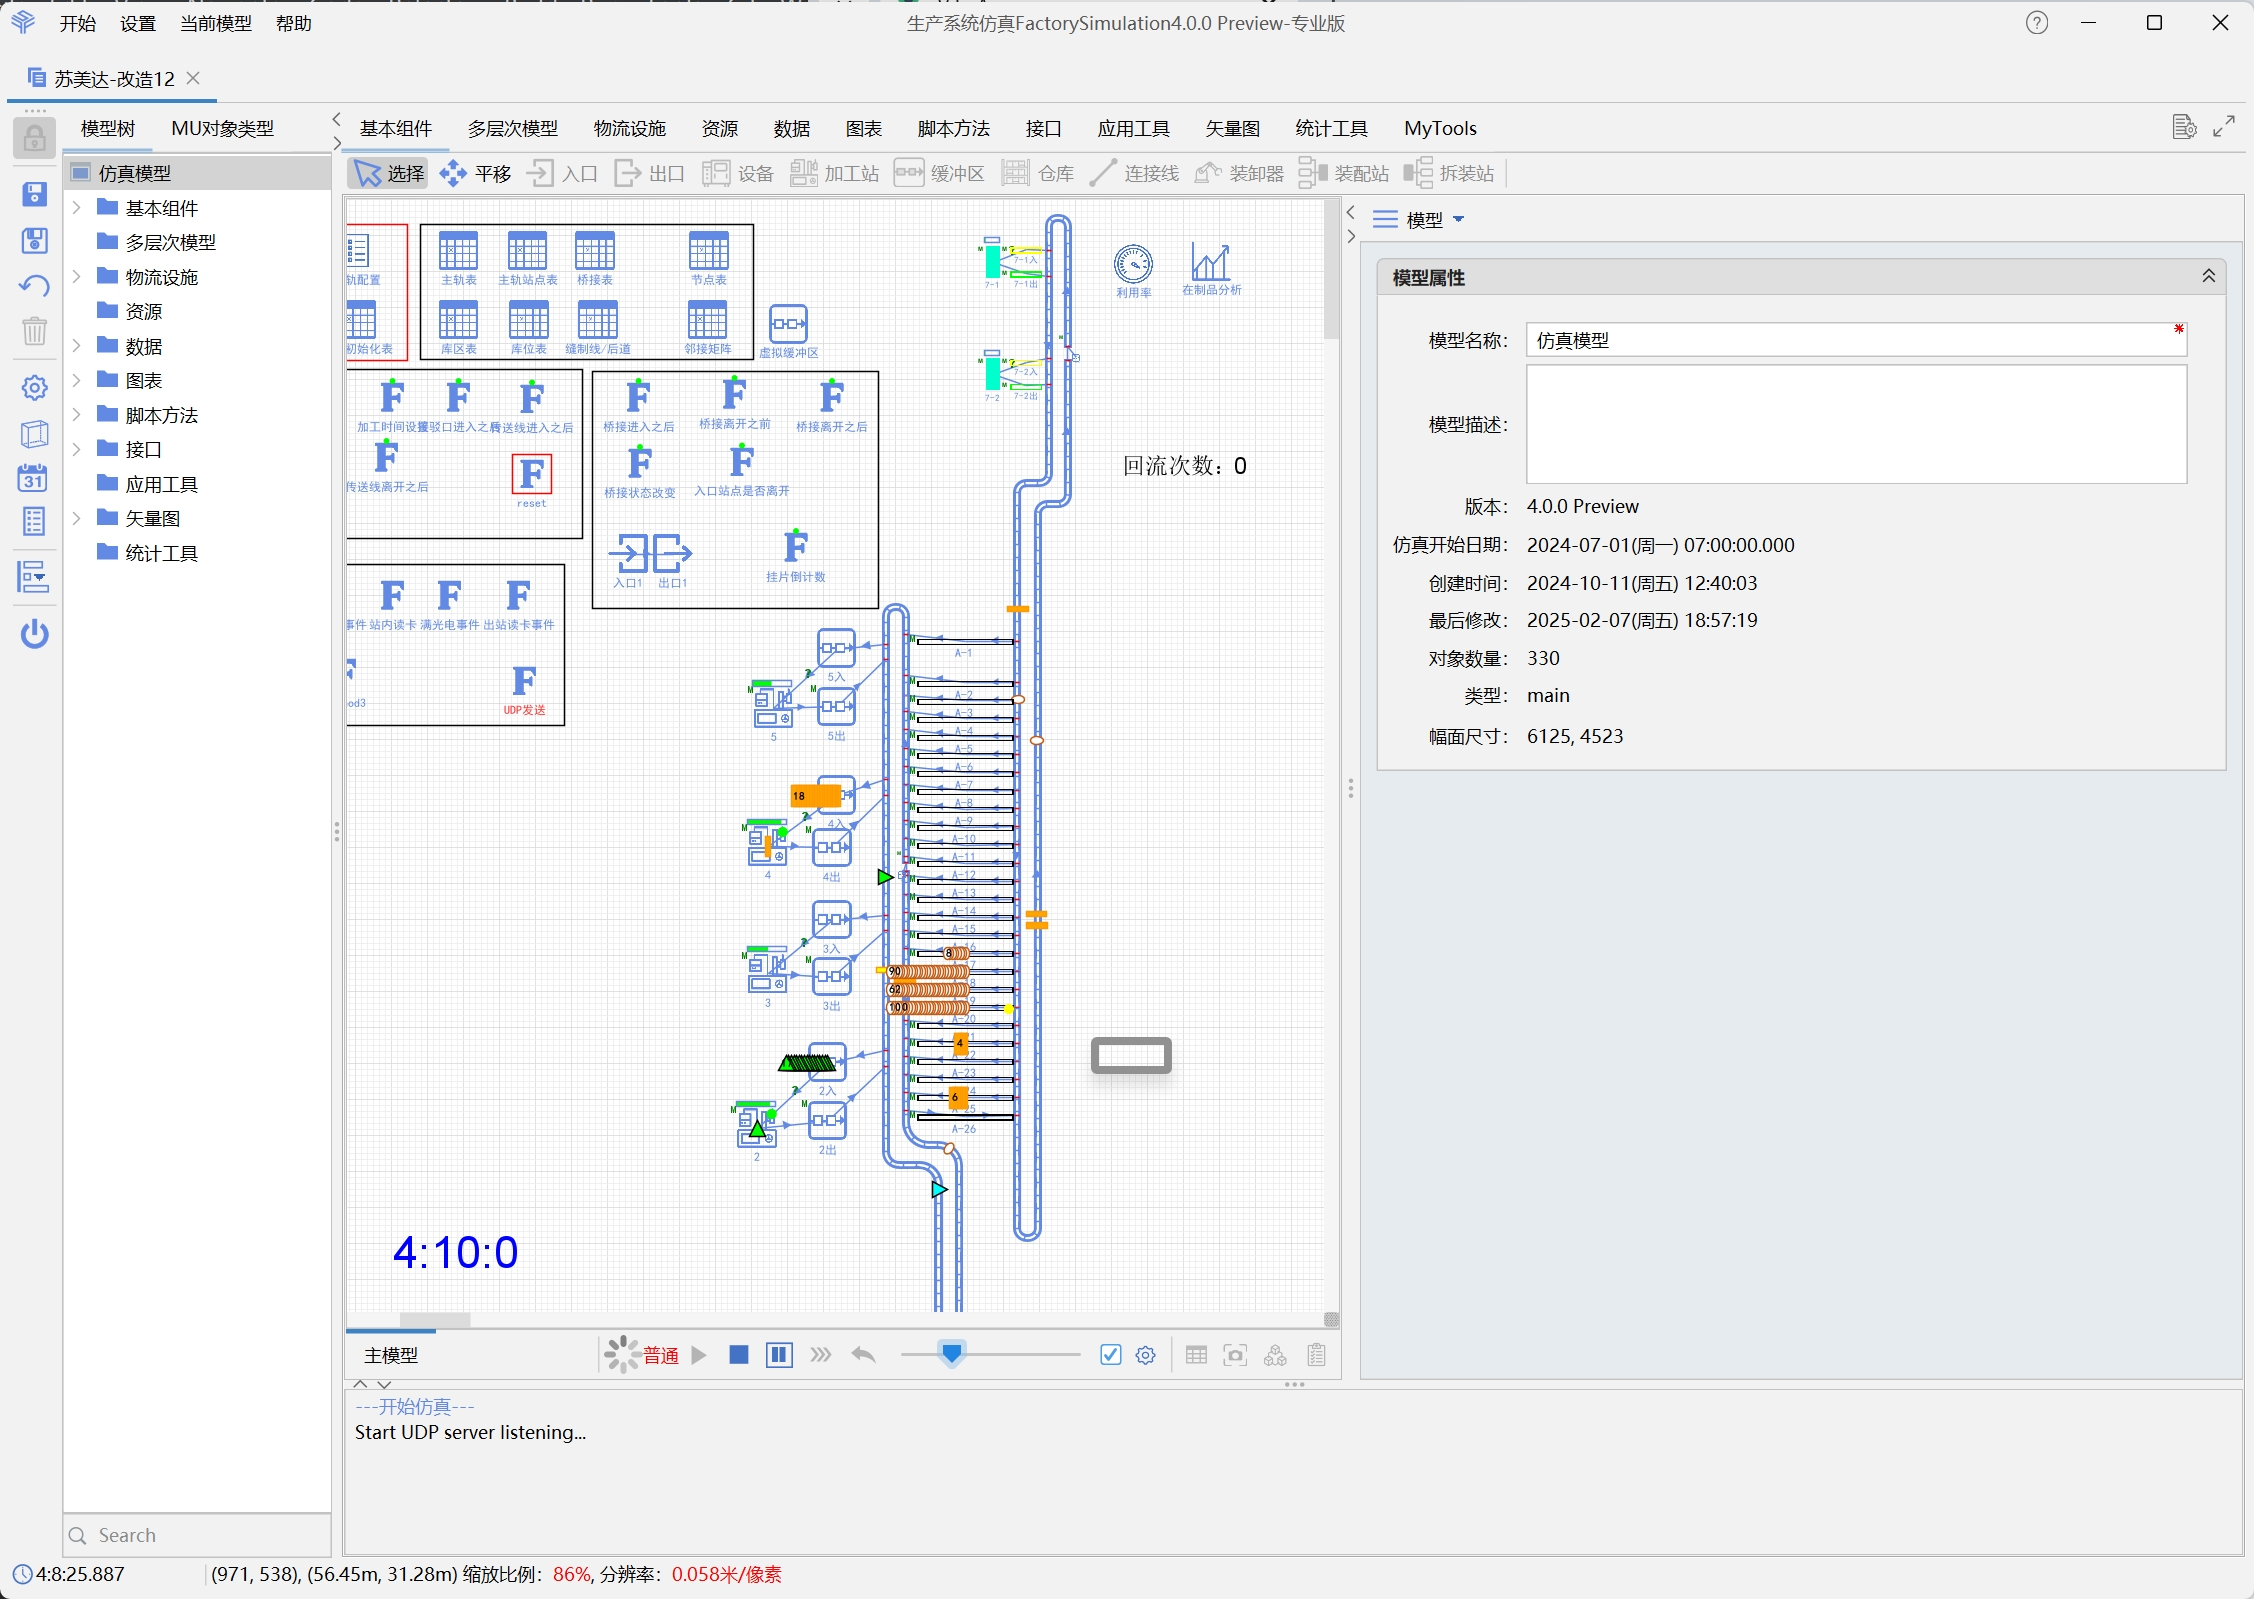
\includegraphics[width=0.9\textwidth]{pics/jack/jack-fs-sim.jpg}
	\caption{FS模型总览图}\label{fig:jack-fs-sim}
\end{figure}
\subsection{模型场景说明}
如图\ref{fig:jack-fs-sim}所示，FS模型基于苏美达工厂的场景创建，按主轨说明如下：
\begin{enumerate}[label=\hspace{18pt}\arabic*)]
	\item \bf{主轨701}，7号线，包含：
	\begin{itemize}
		\item 两个\it{挂片站}（7-1、7-2）的出入口
		\item \it{A仓} 24根存储杆的入口
		\item 7线$\rightarrow$8线\it{快速通道}入口
		\item 7线$\leftarrow$8线\it{回流通道}出口
	\end{itemize}
	\item \bf{主轨801}，8号线，包含： 
	\begin{itemize}
		\item 两个\it{挂片站}（8-2、8-4）的出入口
		\item \it{A仓} 24根存储杆的出口
		\item 7线$\rightarrow$8线\it{快速通道}出口
		\item 8线$\rightarrow$7线\it{回流通道}入口
		\item 1线$\leftrightarrow$8线\it{桥接通道}出入口
		\item 2线$\leftrightarrow$8线\it{桥接通道}出入口
		\item 3线$\leftrightarrow$8线\it{桥接通道}出入口
		\item 4线$\leftrightarrow$8线\it{桥接通道}出入口
		\item 5线$\leftrightarrow$8线\it{桥接通道}出入口
		\item \it{B仓} 10根存储杆的入口
		\item 8线$\rightarrow$9线\it{快速通道}入口
		\item 8线$\leftarrow$9线\it{回流通道}出口
	\end{itemize}
	\item \bf{主轨101}，1号线，本例简化为1个工站
	\item \bf{主轨201}，2号线，本例简化为1个工站
	\item \bf{主轨301}，3号线，本例简化为1个工站
	\item \bf{主轨401}，4号线，本例简化为1个工站
	\item \bf{主轨501}，5号线，本例简化为1个工站
	\item \bf{主轨601}，6号线，本例略
	\item \bf{主轨9012}，9号线2楼段，包含： 
	\begin{itemize}
		\item \it{B仓} 10根存储杆的出口
		\item 8线$\rightarrow$9线\it{快速通道}出口
		\item 8线$\leftarrow$9线\it{回流通道}入口
	\end{itemize}
	\item \bf{主轨9011}，9号线1楼段，包含： 
	\begin{itemize}
		\item \it{C仓} 15根存储杆的入口
		\item 9线$\rightarrow$10线\it{快速通道}入口
		\item 9线$\leftarrow$10线\it{回流通道}出口
	\end{itemize}
	\item \bf{主轨1001}，10号线，包含： 
	\begin{itemize}
		\item \it{10号线工站} 本例简化为1个工站
		\item \it{C仓} 15根存储杆的出口
		\item 9线$\rightarrow$10线\it{快速通道}出口
		\item 9线$\leftarrow$10线\it{回流通道}入口
	\end{itemize}
\end{enumerate}
\subsection{对象建模}
\begin{enumerate}[label=\hspace{18pt}\arabic*)]
	\item \bf{主轨}：在fs中属于ConveyorLine （传送线），也可以叫 Track（轨道），含若干TrackStation（主轨站点）\footnote{\bf{主轨站点}：不同于工站、存储杆这样的站点概念，轨道站点可理解为主轨上进出工站/存储杆的出入口}，含两个特殊TrackStation，编号为0点线头站点和编号为999的线尾站点。除特殊站点，其它站点可任意命名，但必须唯一。如图\secref{fig:conveyorline}所示。注意事项：
	
	\item \bf{连接线}
	\begin{itemize}
		\item \it{999}$\rightarrow$\it{0}：Connector（连接线），主轨传送线首尾相接的连接线，如图\secref{fig:connector}所示。
		\item \it{主轨站点}$\rightarrow$\it{车缝站入站缓冲区}：Connector（连接线）。
		\item \it{主轨站点}$\rightarrow$\it{存储杆缓冲区}：Connector（连接线）。
		\begin{figure}[H]%[htbp!]
			\centering
			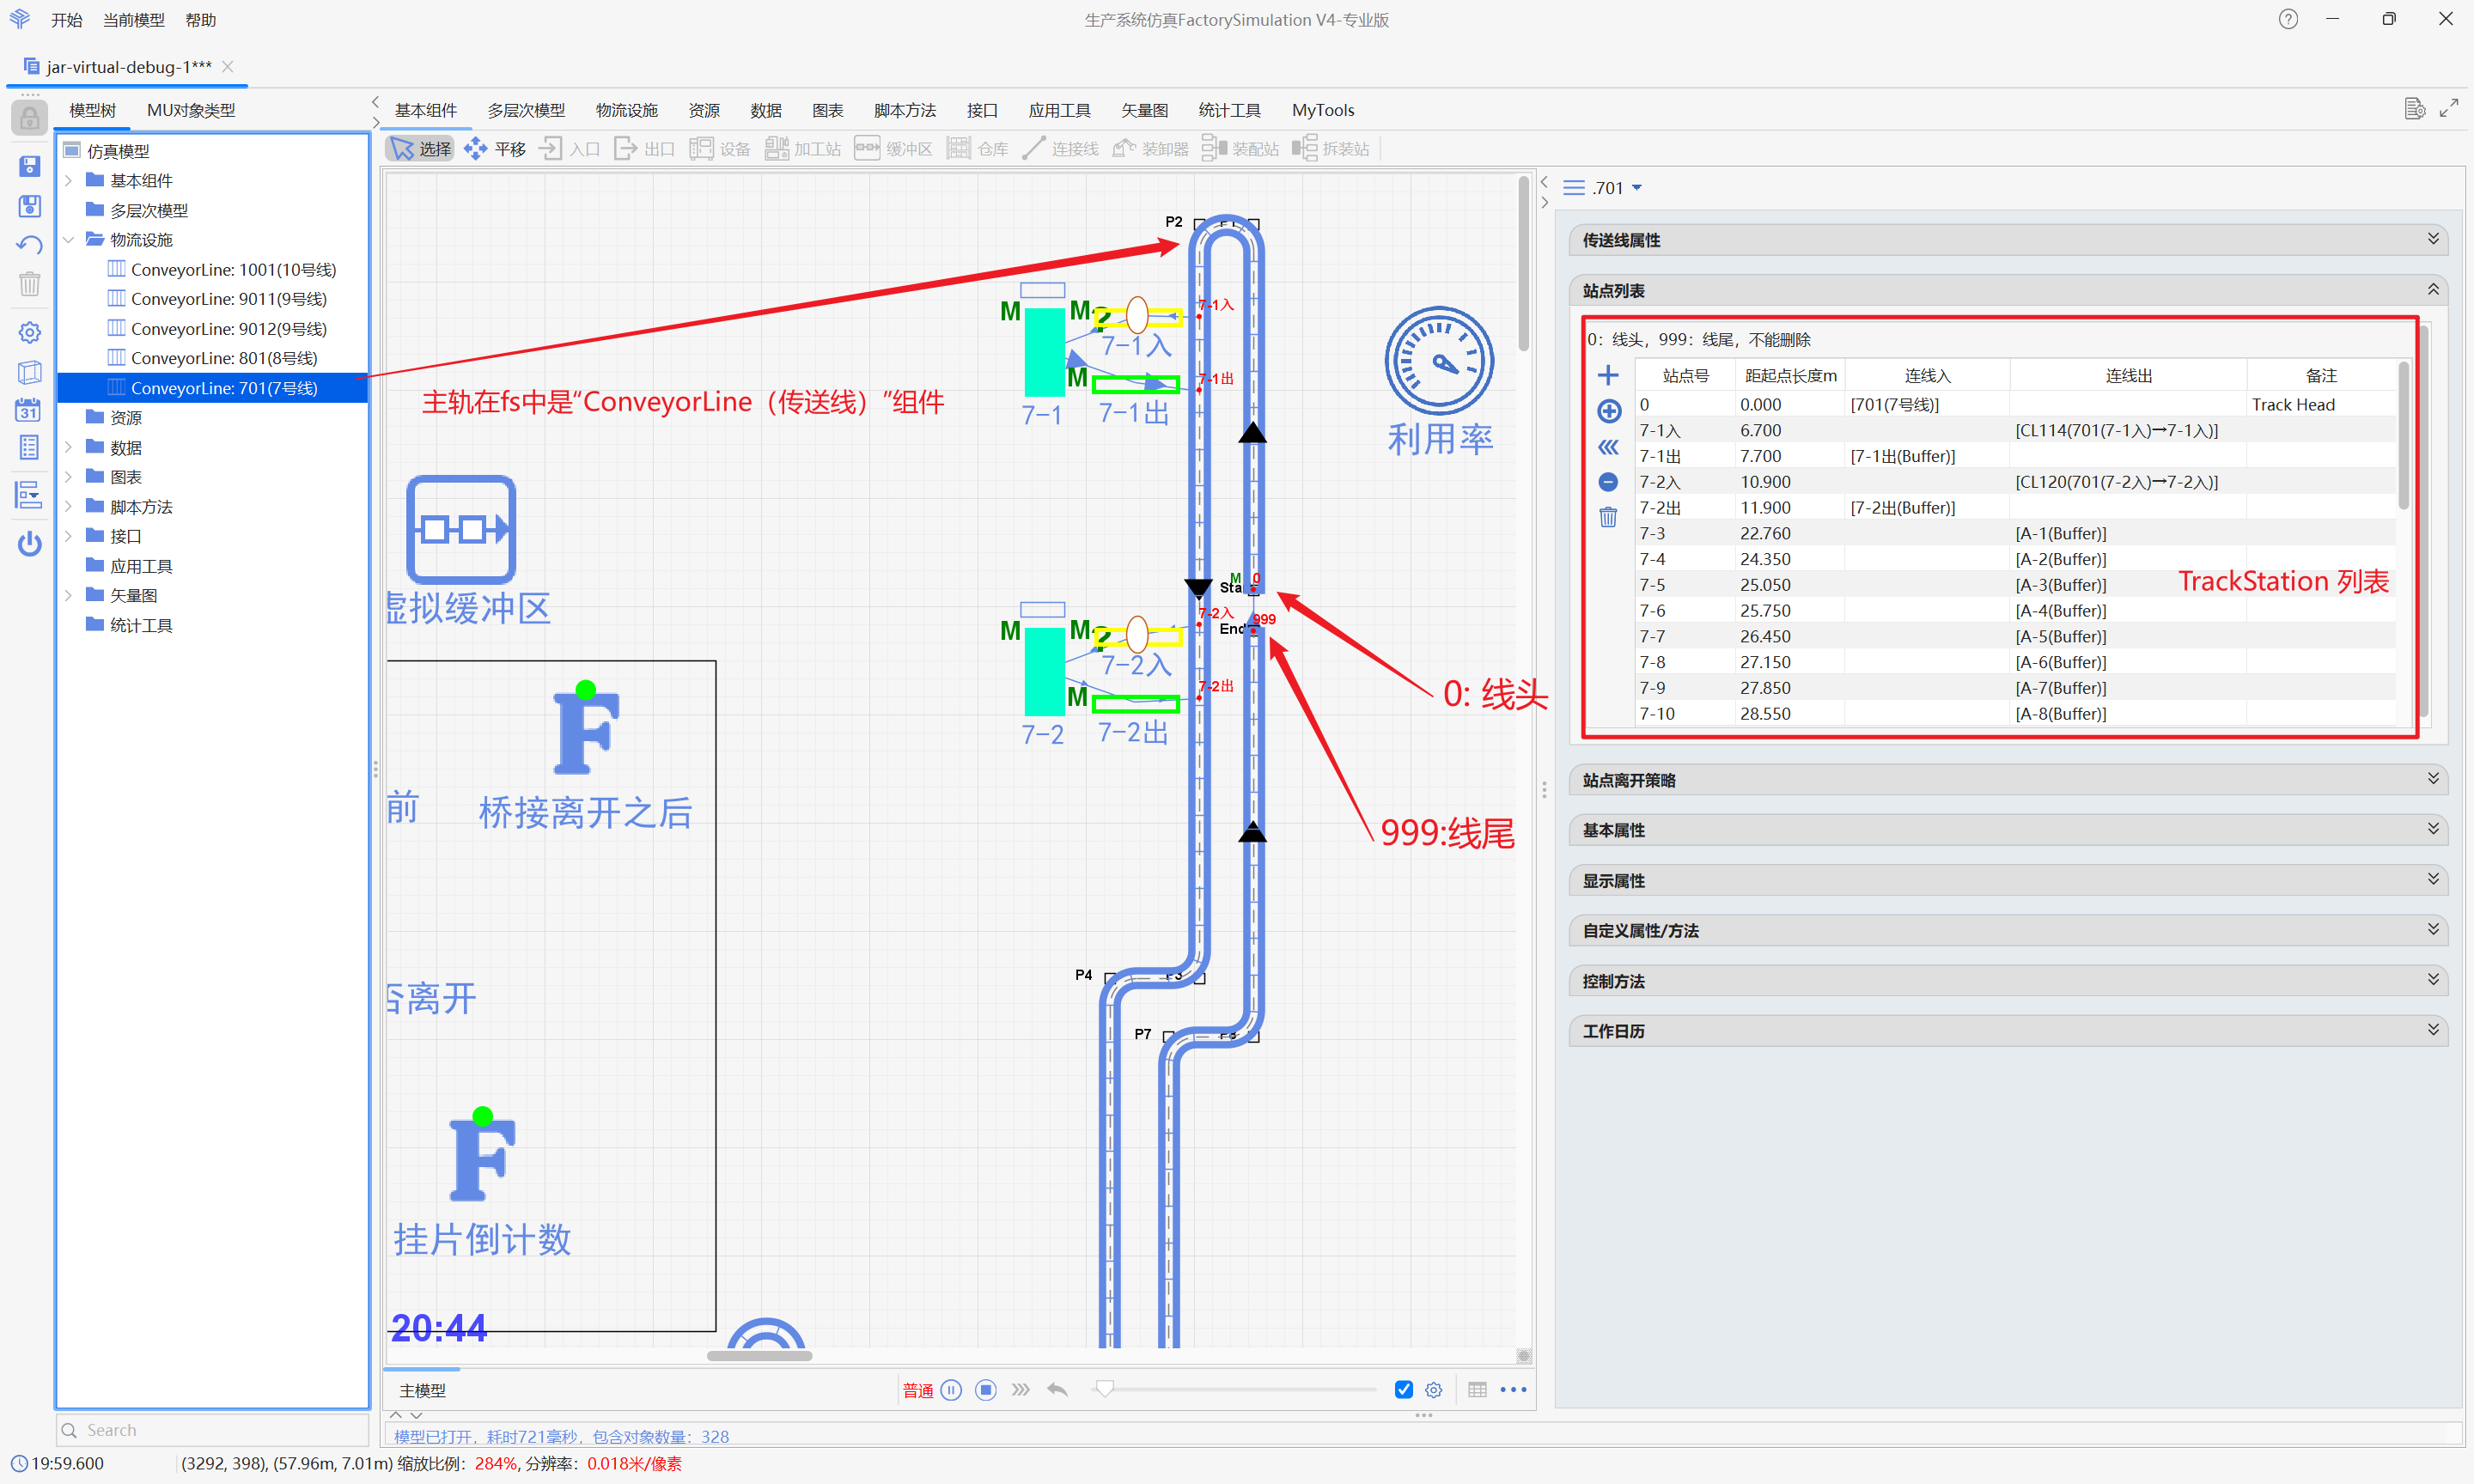
\includegraphics[width=0.9\textwidth]{pics/jack/conveyorline.png}
			\caption{主轨对象模型}
			\label{fig:conveyorline}
		\end{figure}
		\begin{figure}[H]%[htbp!]
			\centering
			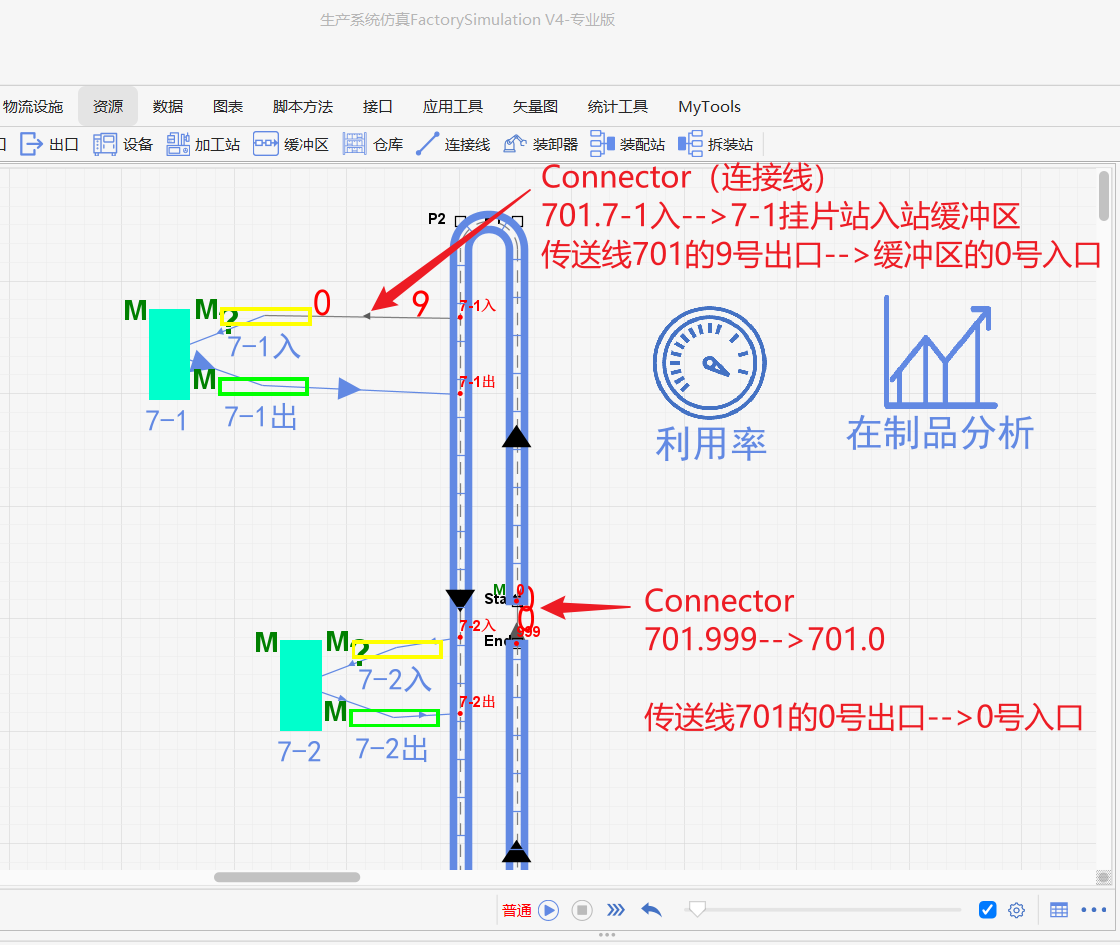
\includegraphics[width=0.7\textwidth]{pics/jack/connector.png}
			\caption{Connector对象模型}
			\label{fig:connector}
		\end{figure}
		\item \it{主轨站点}$\rightarrow$\it{快速通道缓冲区}：Connector（连接线）。
		\item \it{主轨站点}$\leftarrow$\it{回流通道缓冲区}：Connector（连接线）。
	\end{itemize}

	\item \bf{工站}，工站模型由如下组件组成（如图\secref{fig:workstation}）:
	\begin{itemize}
		\item \it{待加工缓存/螺旋弯}：Buffer（缓冲区）。
		\item \it{车缝站/挂片站}：Workstation（工站）。包括车缝站、质检站、挂片站。
		\item \it{出站缓存}：Buffer（缓冲区）。
		\item \it{主轨$\rightarrow$待加工缓存/螺旋弯}：Connector（连接线）。
		\item \it{待加工缓存/螺旋弯$\rightarrow$车缝站/挂片站}：Connector（连接线）。
		\item \it{车缝站/挂片站$\rightarrow$主轨}：Connector（连接线）。
	\end{itemize}
	\begin{figure}[H]%[htbp!]
		\centering
		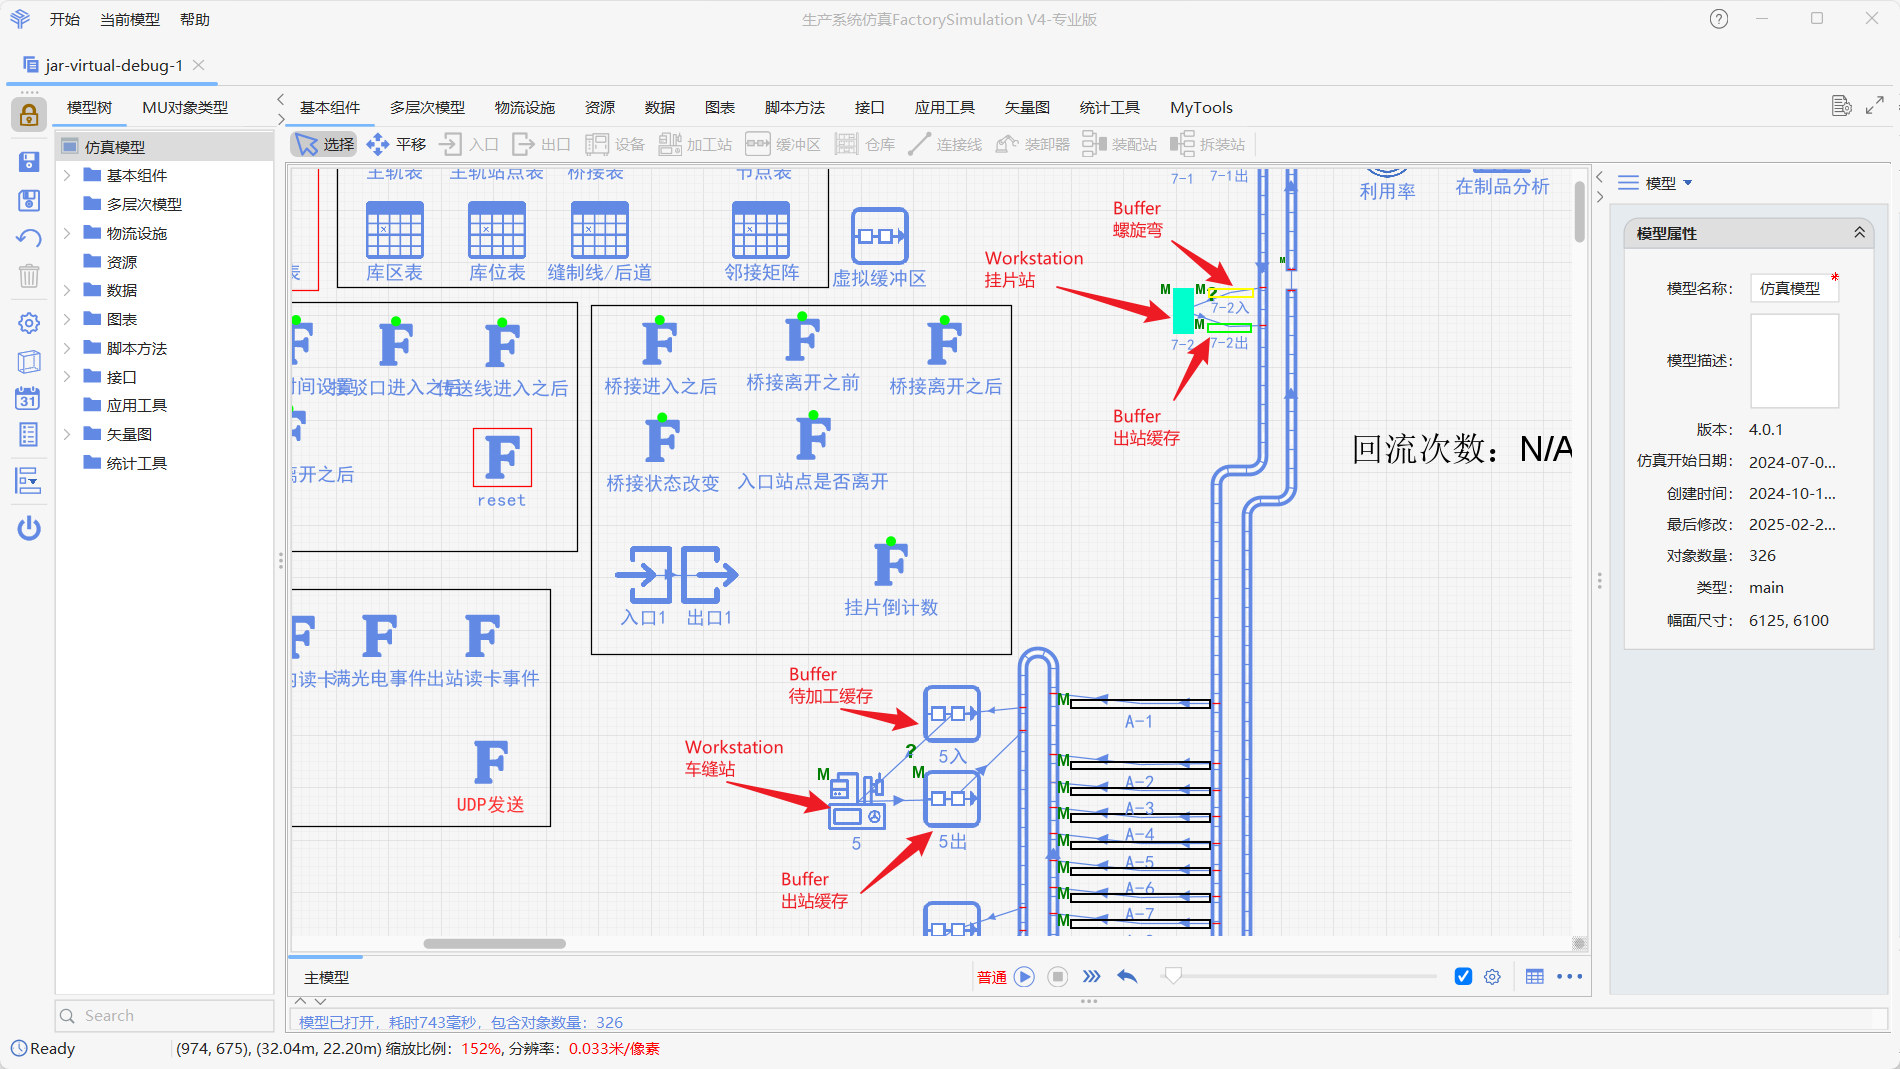
\includegraphics[width=0.7\textwidth]{pics/jack/workstation.png}
		\caption{工站对象模型}
		\label{fig:workstation}
	\end{figure}

	\item \bf{存储杆、快速通道、回流通道}，工站模型由如下组件组成（如图\secref{fig:rod}）：
	\begin{figure}[H]%[htbp!]
		\centering
		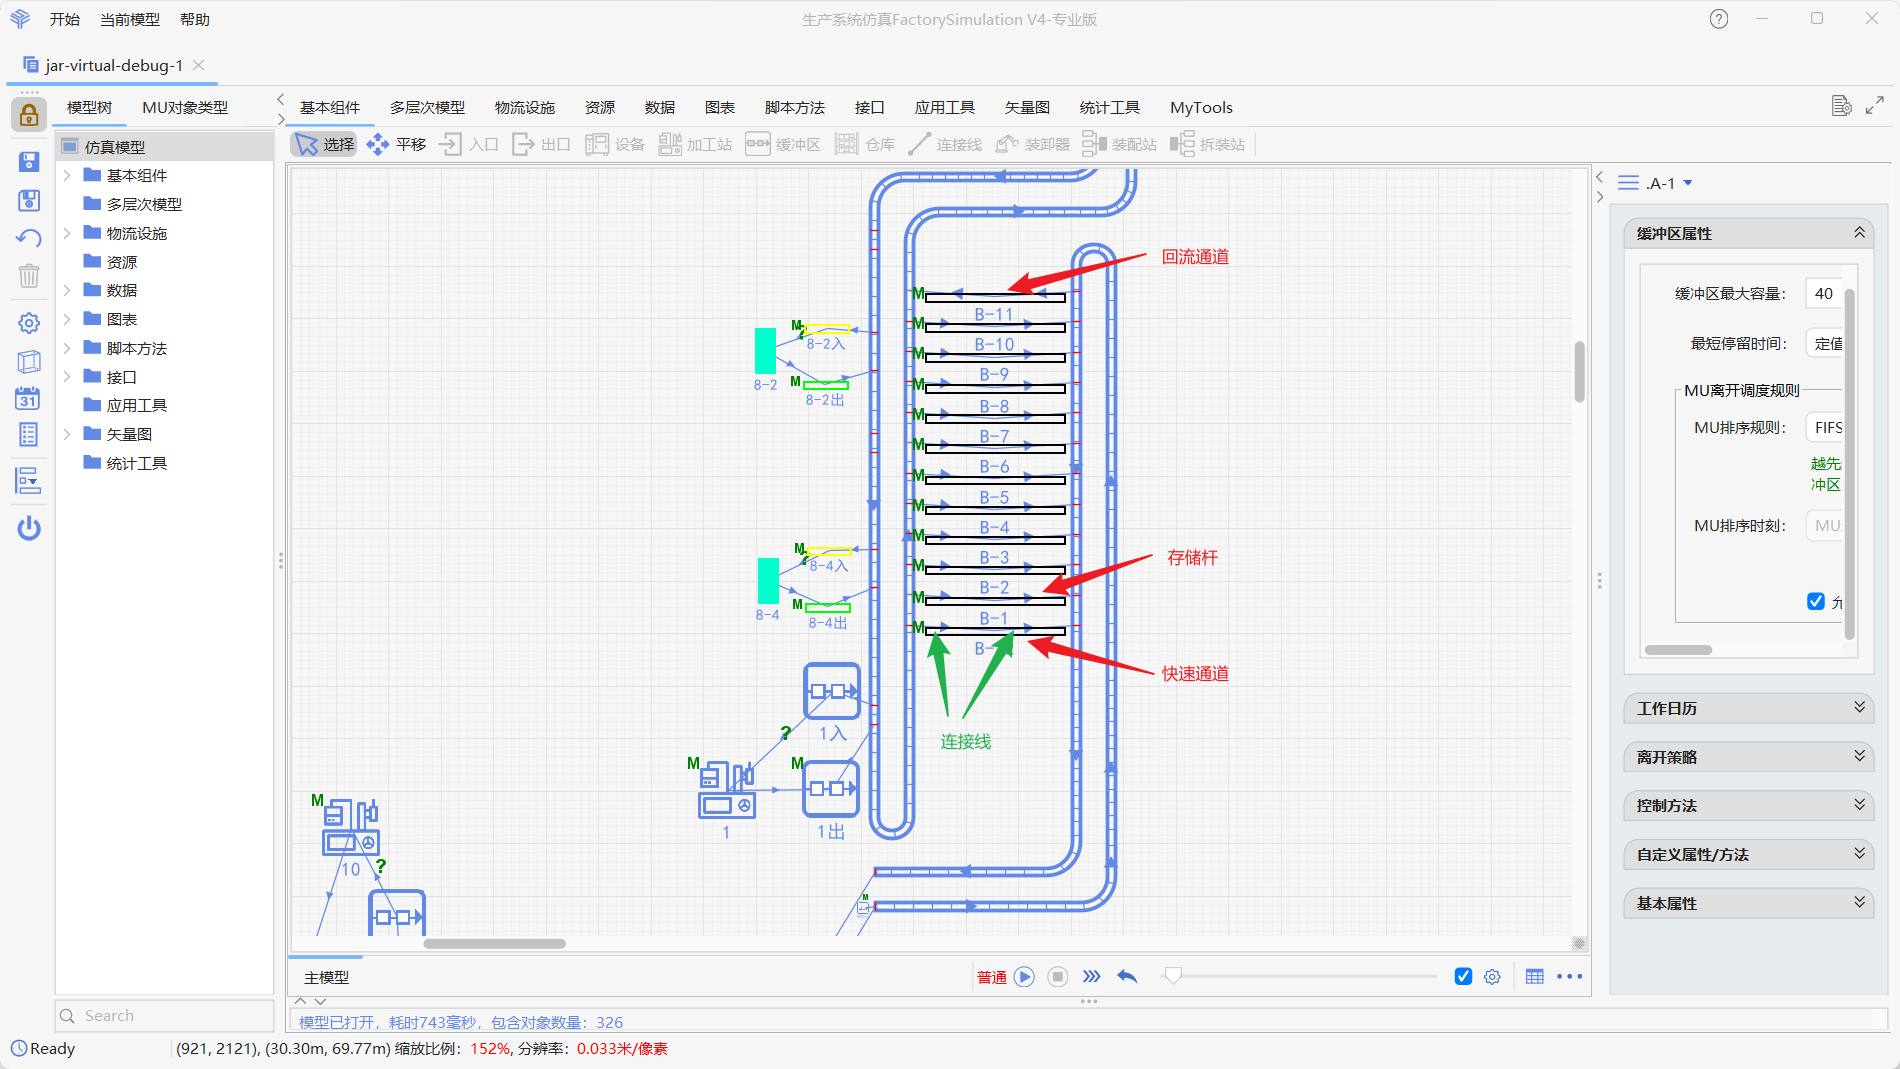
\includegraphics[width=0.7\textwidth]{pics/jack/rod.png}
		\caption{存储杆、快速通道、回流通道}
		\label{fig:rod}
	\end{figure}
	\begin{itemize}
		\item \it{存储杆}：Buffer（缓冲区）。
		\item \it{快速通道}：Buffer（缓冲区）。
		\item \it{回流通道}：Buffer（缓冲区）。
		\item \it{主轨$\rightarrow$缓冲区}：Connector（连接线）。
		\item \it{缓冲区$\rightarrow$主轨}：Connector（连接线）。
	\end{itemize}

	\item \bf{衣架}，包括空衣架、挂片衣架、本成品衣架（经车缝站不同工序）、成品衣架，在fs模型中称为MU（Mobile Unit），为方便目测区分，用不同形状代表不同款号，用不同颜色代表不同工序，衣架模型如图所示：
	\begin{figure}[H]%[htbp!]
		\centering
		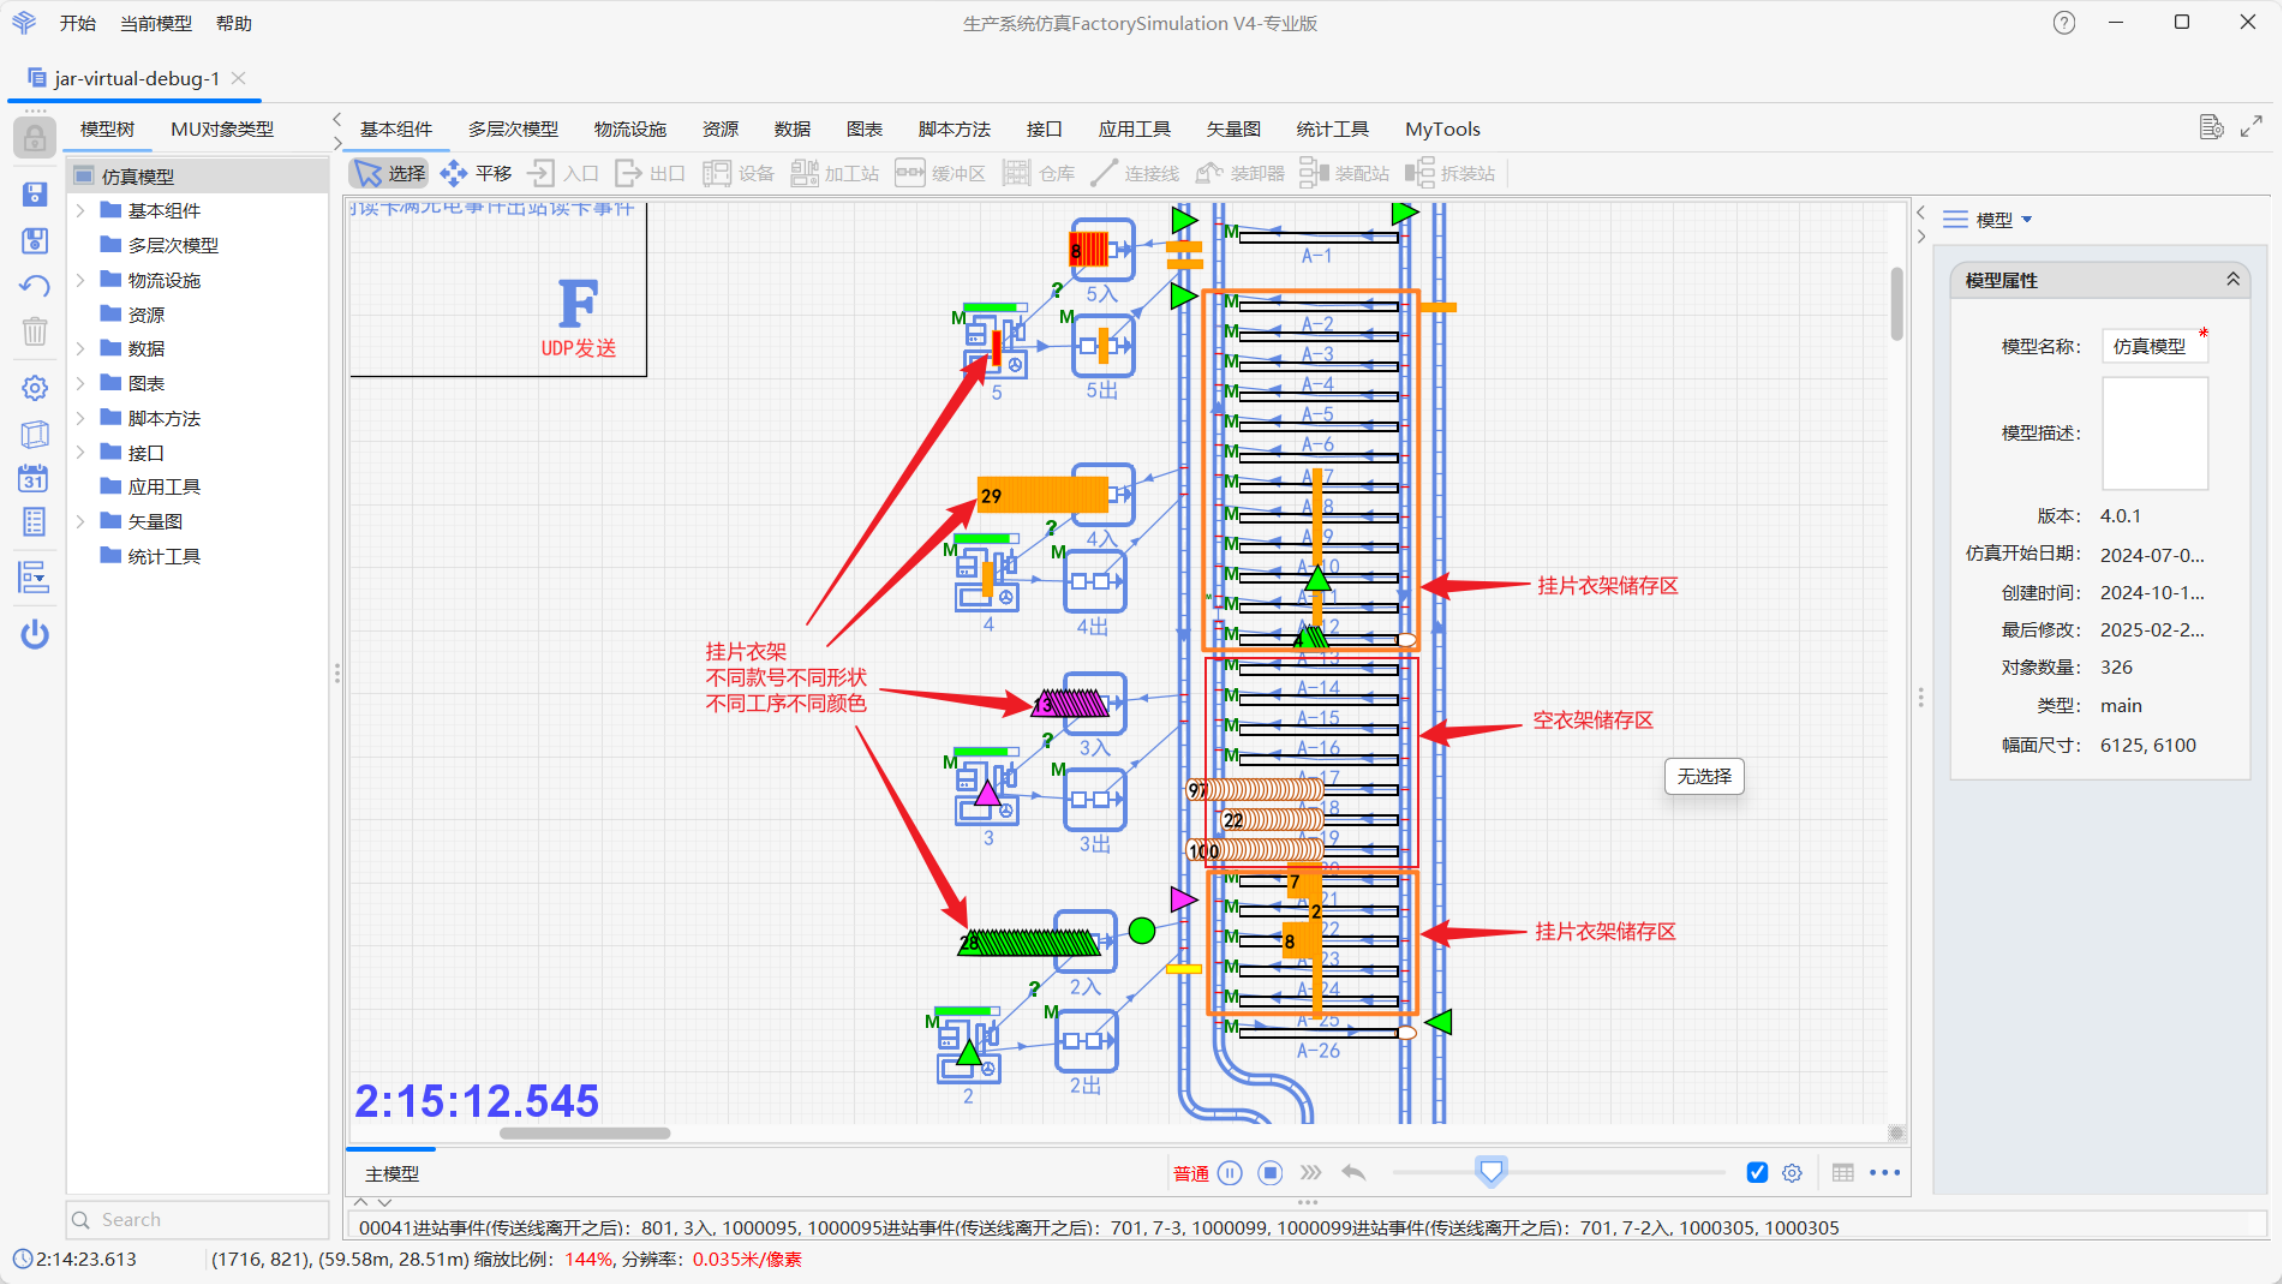
\includegraphics[width=0.7\textwidth]{pics/jack/hanger.png}
		\caption{不同款号、不同工序的衣架}
		\label{fig:hanger}
	\end{figure}
	\begin{figure}[H]%[htbp!]
		\centering
		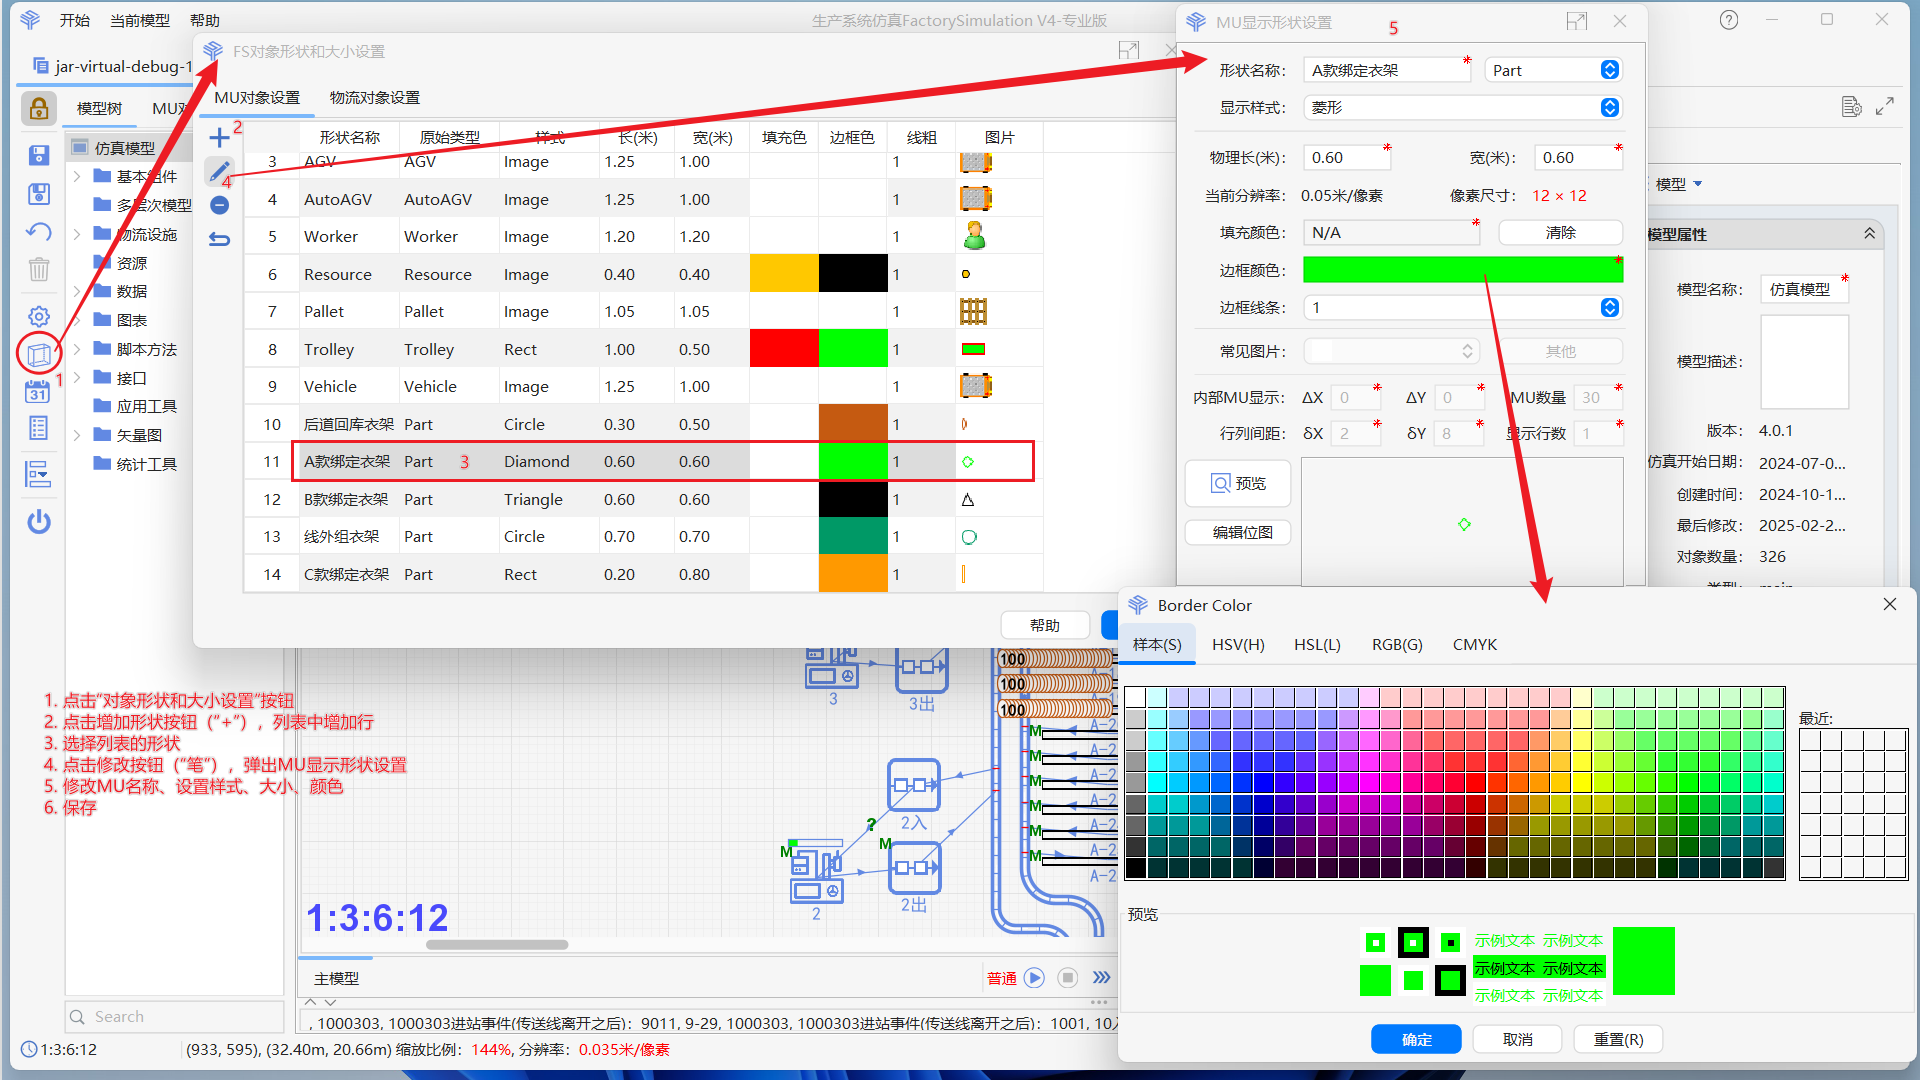
\includegraphics[width=0.7\textwidth]{pics/jack/mustyle.png}
		\caption{设置mu（衣架）形状}
		\label{fig:mu}
	\end{figure}
\end{enumerate}
\subsection{数据建模}
\subsubsection{节点表整理}
	根据对象建模的主轨组件属性，将每条主轨的站点（Trackstation），按逆时针顺序记录编号、上个站点到当前站点的运输耗时（与路径长度对应）等信息。
	\par\tips{初始化的节点表只包含\it{主轨上的站点}，用于路径求解的路网中的节点，除了主轨上的站点，还包含\it{挂片站}、\it{工站}、\it{存储杆}、\it{回流杆}、\it{快速通道}}。

	\begin{center}
	\scriptsize{
		\tablefirsthead{%
			%\toprule[1.5pt]
			\hline
			\head{线号} & \head{主轨号} & \head{节点编号} & \head{节点角色} & \head{序号} & \head{前驱到此时间消耗} & \head{存储类型} & \head{备注} \\
			\hline
			%\midrule
		}
		
		\tablehead{%
			\hline
			\multicolumn{8}{|l|}{\small\sl\textcolor{atomictangerine}{...续前页}}\\
			%\toprule[1.5pt]
			\hline
			%\toprule[1.5pt]
			\head{线号} & \head{主轨号} & \head{节点编号} & \head{节点角色} & \head{序号} & \head{前驱到此时间消耗} & \head{存储类型} & \head{备注} \\
			\hline
			%\midrule
		}
		
		\tabletail{%
			\hline
			\multicolumn{8}{|r|}{\small\sl\textcolor{atomictangerine}{未完待续...}}\\
			\hline
			%\toprule[1.5pt]
		}
		
		\tablelasttail{}
		
		\topcaption{节点表数据}\label{tbl:node-table}
		\begin{supertabular}{|>{\centering}p{8mm}|p{10mm}|p{12mm}|p{18mm}|p{6mm}|p{20mm}|p{30mm}|p{28mm}|}
		7&701&7-1入&入站口&1&213447&STATION-挂片站&空衣架储存区（螺旋弯) \\
		7&701&7-1出&出站口&1&4275&STATION-挂片站&挂片上线 \\
        7 & 701 & 7-2入 & 入站口 & 1 & 12826 & STATION-挂片站 & 空衣架储存区（螺旋弯) \\
        7 & 701 & 7-2出 & 出站口 & 1 & 4275 & STATION-挂片站 & 挂片上线 \\
        7 & 701 & 7-3 & 快速通道上游 & 1 & 49469 & ROD-快速通道 & 去往8线 \\
        7 & 701 & 7-4 & 入杆口 & 1 & 3150 & ROD-存储杆 & A仓 \\
        7 & 701 & 7-5 & 入杆口 & 1 & 3150 & ROD-存储杆 & A仓 \\
        7 & 701 & 7-6 & 入杆口 & 1 & 3150 & ROD-存储杆 & A仓 \\
        7 & 701 & 7-7 & 入杆口 & 1 & 31500 & ROD-存储杆 & A仓 \\
        7 & 701 & 7-8 & 入杆口 & 1 & 31500 & ROD-存储杆 & A仓 \\
        7 & 701 & 7-9 & 入杆口 & 1 & 31500 & ROD-存储杆 & A仓 \\
        7 & 701 & 7-10 & 入杆口 & 1 & 3150 & ROD-存储杆 & A仓 \\
        7 & 701 & 7-11 & 入杆口 & 1 & 3150 & ROD-存储杆 & A仓 \\
        7 & 701 & 7-12 & 入杆口 & 1 & 3150 & ROD-存储杆 & A仓 \\
        7 & 701 & 7-13 & 入杆口 & 1 & 3150 & ROD-存储杆 & A仓 \\
        7 & 701 & 7-14 & 入杆口 & 1 & 3150 & ROD-存储杆 & A仓 \\
        7 & 701 & 7-15 & 入杆口 & 1 & 3150 & ROD-存储杆 & A仓 \\
        7 & 701 & 7-16 & 入杆口 & 1 & 3150 & ROD-空衣架存储杆 & A仓 \\
        7 & 701 & 7-17 & 入杆口 & 1 & 3150 & ROD-空衣架存储杆 & A仓 \\
        7 & 701 & 7-18 & 入杆口 & 1 & 3150 & ROD-空衣架存储杆 & A仓 \\
        7 & 701 & 7-19 & 入杆口 & 1 & 3150 & ROD-空衣架存储杆 & A仓 \\
        7 & 701 & 7-20 & 入杆口 & 1 & 3150 & ROD-空衣架存储杆 & A仓 \\
        7 & 701 & 7-21 & 入杆口 & 1 & 3150 & ROD-空衣架存储杆 & A仓 \\
        7 & 701 & 7-22 & 入杆口 & 1 & 3150 & ROD-空衣架存储杆 & A仓 \\
        7 & 701 & 7-23 & 入杆口 & 1 & 3150 & ROD-存储杆 & A仓 \\
        7 & 701 & 7-24 & 入杆口 & 1 & 3150 & ROD-存储杆 & A仓 \\
        7 & 701 & 7-25 & 入杆口 & 1 & 3150 & ROD-存储杆 & A仓 \\
        7 & 701 & 7-26 & 入杆口 & 1 & 3150 & ROD-存储杆 & A仓 \\
        7 & 701 & 7-27 & 入杆口 & 1 & 3150 & ROD-存储杆 & A仓 \\
        7 & 701 & 7-28 & 回流通道下游 & 1 & 3150 & ROD-回流通道 & 来自8线 \\
		\hline
        8 & 801 & 8-1入 & 入站口 & 1 & 119711 & STATION-空衣架回收站 &  \\
        8 & 801 & 8-1出 & 出站口 & 1 & 4275 & STATION-空衣架回收站 &  \\
        8 & 801 & 8-2入 & 入站口 & 1 & 8775 & STATION-挂片站 &  \\
        8 & 801 & 8-2出 & 出站口 & 1 & 4275 & STATION-挂片站 &  \\
        8 & 801 & 8-3入 & 入站口 & 1 & 5954 & STATION-空衣架回收站 &  \\
        8 & 801 & 8-3出 & 出站口 & 1 & 4275 & STATION-空衣架回收站 &  \\
        8 & 801 & 8-4入 & 入站口 & 1 & 10572 & STATION-挂片站 &  \\
        8 & 801 & 8-4出 & 出站口 & 1 & 4275 & STATION-挂片站 &  \\
        8 & 801 & 1入 & 入站口 & 1 & 27329 & STATION-加工站 &  \\
        8 & 801 & 1出 & 出站口 & 1 & 3060 & STATION-加工站 &  \\
        8 & 801 & 8-6 & 快速通道上游 & 1 & 24451 & ROD-快速通道 & 去往9012线 \\
        8 & 801 & 8-7 & 出杆口 & 1 & 3600 & ROD-存储杆 & A仓 \\
        8 & 801 & 8-8 & 出杆口 & 1 & 3600 & ROD-存储杆 & A仓 \\
        8 & 801 & 8-9 & 出杆口 & 1 & 3600 & ROD-存储杆 & A仓 \\
        8 & 801 & 8-10 & 出杆口 & 1 & 3600 & ROD-存储杆 & A仓 \\
        8 & 801 & 8-11 & 出杆口 & 1 & 3600 & ROD-存储杆 & A仓 \\
        8 & 801 & 8-12 & 出杆口 & 1 & 3600 & ROD-存储杆 & A仓 \\
        8 & 801 & 8-13 & 出杆口 & 1 & 3600 & ROD-存储杆 & A仓 \\
        8 & 801 & 8-14 & 出杆口 & 1 & 3600 & ROD-存储杆 & A仓 \\
        8 & 801 & 8-15 & 出杆口 & 1 & 3600 & ROD-存储杆 & A仓 \\
        8 & 801 & 8-16 & 出杆口 & 1 & 3600 & ROD-存储杆 & A仓 \\
        8 & 801 & 8-17 & 回流通道下游 & 1 & 3600 & ROD-回流通道 & 来自9012线 \\
        8 & 801 & 8-47 & 回流通道上游 & 1 & 115301 & ROD-回流通道 & 去往7线 \\
        8 & 801 & 8-18 & 出杆口 & 1 & 3150 & ROD-存储杆 & A仓 \\
        8 & 801 & 8-19 & 出杆口 & 1 & 3150 & ROD-存储杆 & A仓 \\
        8 & 801 & 8-20 & 出杆口 & 1 & 3150 & ROD-存储杆 & A仓 \\
        8 & 801 & 8-21 & 出杆口 & 1 & 3150 & ROD-存储杆 & A仓 \\
        8 & 801 & 8-22 & 出杆口 & 1 & 3150 & ROD-存储杆 & A仓 \\
        8 & 801 & 8-23 & 出杆口 & 1 & 3150 & ROD-空衣架存储杆 & A仓 \\
        8 & 801 & 8-24 & 出杆口 & 1 & 3150 & ROD-空衣架存储杆 & A仓 \\
        8 & 801 & 8-25 & 出杆口 & 1 & 3150 & ROD-空衣架存储杆 & A仓 \\
        8 & 801 & 8-26 & 出杆口 & 1 & 3150 & ROD-空衣架存储杆 & A仓 \\
        8 & 801 & 8-27 & 出杆口 & 1 & 3150 & ROD-空衣架存储杆 & A仓 \\
        8 & 801 & 8-28 & 出杆口 & 1 & 3150 & ROD-空衣架存储杆 & A仓 \\
        8 & 801 & 8-29 & 出杆口 & 1 & 3150 & ROD-空衣架存储杆 & A仓 \\
        8 & 801 & 8-30 & 出杆口 & 1 & 3150 & ROD-存储杆 & A仓 \\
        8 & 801 & 8-31 & 出杆口 & 1 & 3150 & ROD-存储杆 & A仓 \\
        8 & 801 & 8-32 & 出杆口 & 1 & 3150 & ROD-存储杆 & A仓 \\
        8 & 801 & 8-33 & 出杆口 & 1 & 3150 & ROD-存储杆 & A仓 \\
        8 & 801 & 8-34 & 出杆口 & 1 & 3150 & ROD-存储杆 & A仓 \\
        8 & 801 & 8-35 & 出杆口 & 1 & 3150 & ROD-存储杆 & A仓 \\
        8 & 801 & 8-36 & 出杆口 & 1 & 3150 & ROD-存储杆 & A仓 \\
        8 & 801 & 8-37 & 出杆口 & 1 & 3150 & ROD-存储杆 & A仓 \\
        8 & 801 & 8-38 & 出杆口 & 1 & 3150 & ROD-存储杆 & A仓 \\
        8 & 801 & 8-39 & 出杆口 & 1 & 3150 & ROD-存储杆 & A仓 \\
        8 & 801 & 8-40 & 出杆口 & 1 & 3150 & ROD-存储杆 & A仓 \\
        8 & 801 & 8-41 & 出杆口 & 1 & 3150 & ROD-存储杆 & A仓 \\
        8 & 801 & 8-42 & 快速通道下游 & 1 & 3150 & ROD-快速通道 & 来自7线 \\
        8 & 801 & 5入 & 入站口 & 1 & 15752 & STATION-加工站 &  \\
        8 & 801 & 5出 & 出站口 & 1 & 3600 & STATION-加工站 &  \\
        8 & 801 & 4入 & 入站口 & 1 & 29928 & STATION-加工站 &  \\
        8 & 801 & 4出 & 出站口 & 1 & 3600 & STATION-加工站 &  \\
        8 & 801 & 3入 & 入站口 & 1 & 25653 & STATION-加工站 &  \\
        8 & 801 & 3出 & 出站口 & 1 & 3600 & STATION-加工站 &  \\
        8 & 801 & 2入 & 入站口 & 1 & 26103 & STATION-加工站 &  \\
        8 & 801 & 2出 & 出站口 & 1 & 3600 & STATION-加工站 &  \\
		\hline
        9 & 9012 & 9-1 & 快速通道下游 & 1 & 3600 & ROD-快速通道 & 来自8线 \\
        9 & 9011 & 9-29 & 快速通道上游 & 1 & 72615 & ROD-快速通道 & C仓 \\
        9 & 9011 & 9-28 & 入杆口 & 1 & 3600 & ROD-存储杆 & C仓 \\
        9 & 9011 & 9-27 & 入杆口 & 1 & 3600 & ROD-存储杆 & C仓 \\
        9 & 9011 & 9-26 & 入杆口 & 1 & 3600 & ROD-存储杆 & C仓 \\
        9 & 9011 & 9-25 & 入杆口 & 1 & 3600 & ROD-存储杆 & C仓 \\
        9 & 9011 & 9-24 & 入杆口 & 1 & 3600 & ROD-存储杆 & C仓 \\
        9 & 9011 & 9-23 & 入杆口 & 1 & 3600 & ROD-存储杆 & C仓 \\
        9 & 9011 & 9-22 & 入杆口 & 1 & 3600 & ROD-存储杆 & C仓 \\
        9 & 9011 & 9-21 & 入杆口 & 1 & 3600 & ROD-存储杆 & C仓 \\
        9 & 9011 & 9-20 & 入杆口 & 1 & 3600 & ROD-存储杆 & C仓 \\
        9 & 9011 & 9-19 & 入杆口 & 1 & 3600 & ROD-存储杆 & C仓 \\
        9 & 9011 & 9-18 & 入杆口 & 1 & 3600 & ROD-存储杆 & C仓 \\
        9 & 9011 & 9-17 & 入杆口 & 1 & 3600 & ROD-存储杆 & C仓 \\
        9 & 9011 & 9-16 & 入杆口 & 1 & 3600 & ROD-存储杆 & C仓 \\
        9 & 9011 & 9-15 & 入杆口 & 1 & 3600 & ROD-存储杆 & C仓 \\
        9 & 9011 & 9-14 & 入杆口 & 1 & 3600 & ROD-存储杆 & C仓 \\
        9 & 9011 & 9-13 & 回流通道下游 & 1 & 6301 & ROD-回流通道 & 来自10线 \\
        9 & 9012 & 9-12 & 回流通道上游 & 1 & 207588 & ROD-回流通道 & 去往8线 \\
        9 & 9012 & 9-11 & 出杆口 & 1 & 6301 & ROD-存储杆 & B仓 \\
        9 & 9012 & 9-10 & 出杆口 & 1 & 3600 & ROD-存储杆 & B仓 \\
        9 & 9012 & 9-9 & 出杆口 & 1 & 3600 & ROD-存储杆 & B仓 \\
        9 & 9012 & 9-8 & 出杆口 & 1 & 3600 & ROD-存储杆 & B仓 \\
        9 & 9012 & 9-7 & 出杆口 & 1 & 3600 & ROD-存储杆 & B仓 \\
        9 & 9012 & 9-6 & 出杆口 & 1 & 3600 & ROD-存储杆 & B仓 \\
        9 & 9012 & 9-5 & 出杆口 & 1 & 3600 & ROD-存储杆 & B仓 \\
        9 & 9012 & 9-4 & 出杆口 & 1 & 3600 & ROD-存储杆 & B仓 \\
        9 & 9012 & 9-3 & 出杆口 & 1 & 3600 & ROD-存储杆 & B仓 \\
        9 & 9012 & 9-2 & 出杆口 & 1 & 3600 & ROD-存储杆 & B仓 \\
		\hline
        10 & 1001 & 10入 & 入站口 & 1 & 21985 & STATION-加工站 &  \\
        10 & 1001 & 10出 & 出站口 & 1 & 3060 & STATION-加工站 &  \\
        10 & 1001 & 10-7 & 回流通道上游 & 1 & 122412 & ROD-回流通道 & 去往9011线 \\
        10 & 1001 & 10-8 & 出杆口 & 1 & 6301 & ROD-存储杆 & C仓 \\
        10 & 1001 & 10-9 & 出杆口 & 1 & 3600 & ROD-存储杆 & C仓 \\
        10 & 1001 & 10-10 & 出杆口 & 1 & 3600 & ROD-存储杆 & C仓 \\
        10 & 1001 & 10-11 & 出杆口 & 1 & 3600 & ROD-存储杆 & C仓 \\
        10 & 1001 & 10-12 & 出杆口 & 1 & 3600 & ROD-存储杆 & C仓 \\
        10 & 1001 & 10-13 & 出杆口 & 1 & 3600 & ROD-存储杆 & C仓 \\
        10 & 1001 & 10-14 & 出杆口 & 1 & 3600 & ROD-存储杆 & C仓 \\
        10 & 1001 & 10-15 & 出杆口 & 1 & 3600 & ROD-存储杆 & C仓 \\
        10 & 1001 & 10-16 & 出杆口 & 1 & 3600 & ROD-存储杆 & C仓 \\
        10 & 1001 & 10-17 & 出杆口 & 1 & 3600 & ROD-存储杆 & C仓 \\
        10 & 1001 & 10-18 & 出杆口 & 1 & 3600 & ROD-存储杆 & C仓 \\
        10 & 1001 & 10-19 & 出杆口 & 1 & 3600 & ROD-存储杆 & C仓 \\
        10 & 1001 & 10-20 & 出杆口 & 1 & 3600 & ROD-存储杆 & C仓 \\
        10 & 1001 & 10-21 & 出杆口 & 1 & 3600 & ROD-存储杆 & C仓 \\
        10 & 1001 & 10-22 & 出杆口 & 1 & 3600 & ROD-存储杆 & C仓 \\
        10 & 1001 & 10-23 & 快速通道下游 & 1 & 3600 & ROD-快速通道 & 来自9011线 \\

		\hline
					%\bottomrule[1.5pt]
				\end{supertabular}
			}
		\end{center}


	\subsubsection{桥接表整理}
	包含快速通道和回流通道，表属性为：入口线号、入口主轨号、入口主轨站点编号、出口线号、出口主轨编号、出口主轨站点编号。
	\begin{center}
	\scriptsize{
		\tablefirsthead{%
			%\toprule[1.5pt]
			\hline
			\head{入口线号} & \head{入口主轨号} & \head{入口主轨站点编号} & \head{出口线号} & \head{出口主轨编号} & \head{出口主轨站点编号} \\
			\hline
			%\midrule
		}
		
		\tablehead{%
			\hline
			\multicolumn{6}{|l|}{\small\sl\textcolor{atomictangerine}{...续前页}}\\
			%\toprule[1.5pt]
			\hline
			%\toprule[1.5pt]
			\head{入口线号} & \head{入口主轨号} & \head{入口主轨站点编号} & \head{出口线号} & \head{出口主轨编号} & \head{出口主轨站点编号} \\
			\hline
			%\midrule
		}
		
		\tabletail{%
			\hline
			\multicolumn{6}{|r|}{\small\sl\textcolor{atomictangerine}{未完待续...}}\\
			\hline
			%\toprule[1.5pt]
		}
		
		\tablelasttail{}
		
		\topcaption{桥接表}\label{tbl:bridge-table}
		\begin{supertabular}{|>{\centering}p{20mm}|p{20mm}|p{20mm}|>{\centering}p{20mm}|p{20mm}|p{20mm}|}
        7 & 701 & 3 & 8 & 801 & 42 \\ 
        8 & 801 & 47 & 7 & 701 & 28 \\ 
        9 & 9012 & 12 & 8 & 801 & 17 \\ 
        8 & 801 & 6 & 9 & 9012 & 1 \\ 
        9 & 9011 & 29 & 10 & 1001 & 23 \\ 
        10 & 1001 & 7 & 9 & 901 & 13 \\ 


		\hline
					%\bottomrule[1.5pt]
				\end{supertabular}
			}
		\end{center}

	\subsubsection{库区存储杆模型组件的自定义属性}
	自定义属性\footnote{\bf{自定义属性}：User Attribites，和组件固有属性一起，组成组件在仿真中可使用的属性。可在模型编辑时添加并赋初值，也可在运行态由控制方法（函数）添加或修改。}可以在fs的模型编辑器中进行设置，如表\secref{fig:stockarea-user-attributes}所示。入可以在fs的控制方法中设置和修改，例如init（详见\secref{sec:active-model:init}）方法中的setAttribute()语句都是设置或修改自定义变量。

	由于本文中的FS建模是用于虚拟调试的，大部分控制方法以及自定义属性都大幅简化了，有的自定义属性可能是多余的，只作为参考，不过这类属性对虚拟调试没有影响。具体使用时可忽略或进行删减。
	\begin{figure}[H]%[htbp!]
		\centering
		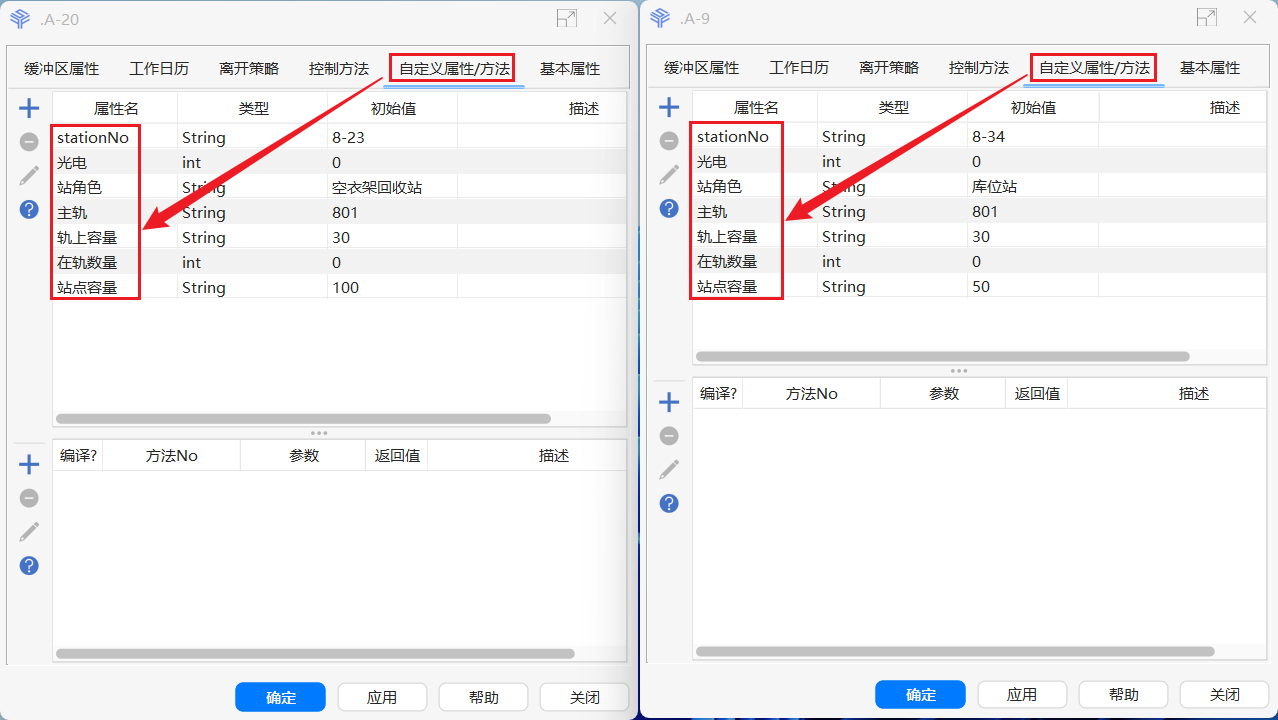
\includegraphics[width=0.7\textwidth]{pics/jack/stockarea_user_attribites.png}
		\caption{存储杆自定义属性}
		\label{fig:stockarea-user-attributes}
	\end{figure}

	\subsubsection{库区表整理}
	包含空衣架存储杆、挂片（半成品）存储杆、成品存储杆、待检仓存储杆。表属性为：入口线号、入口主轨号、入口主轨站点编号、出口线号、出口主轨编号、出口主轨站点编号、杆编号、库区号。库区表的整理，如表\secref{tbl:stockarea-table}所示，一方面是确认对象建模的完整性与正确性，另一方面是作为吊挂系统（以及仓规则Jar包）的配置输入。

	\begin{center}
	\scriptsize{
		\tablefirsthead{%
			%\toprule[1.5pt]
			\hline
			\head{入口线号} & \head{入口主轨号} & \head{入口主轨站点编号} & \head{出口线号} & \head{出口主轨编号} & \head{出口主轨站点编号} & \head{杆编号} & \head{库区号} \\
			\hline
			%\midrule
		}
		
		\tablehead{%
			\hline
			\multicolumn{8}{|l|}{\small\sl\textcolor{atomictangerine}{...续前页}}\\
			%\toprule[1.5pt]
			\hline
			%\toprule[1.5pt]
			\head{入口线号} & \head{入口主轨号} & \head{入口主轨站点编号} & \head{出口线号} & \head{出口主轨号} & \head{出口主轨站点编号} & \head{杆编号} & \head{库区号} \\
			\hline
			%\midrule
		}
		
		\tabletail{%
			\hline
			\multicolumn{8}{|r|}{\small\sl\textcolor{atomictangerine}{未完待续...}}\\
			\hline
			%\toprule[1.5pt]
		}
		
		\tablelasttail{}
		
		\topcaption{库区表}\label{tbl:stockarea-table}
		\begin{supertabular}{|>{\centering}p{10mm}|p{16mm}|p{22mm}|>{\centering}p{10mm}|p{16mm}|p{22mm}|p{10mm}|p{10mm}|}
        7 & 701 & 4 & 8 & 801 & 41 & A-2 & A \\ 
        7 & 701 & 5 & 8 & 801 & 40 & A-3 & A \\ 
        7 & 701 & 6 & 8 & 801 & 39 & A-4 & A \\ 
        7 & 701 & 7 & 8 & 801 & 38 & A-5 & A \\ 
        7 & 701 & 8 & 8 & 801 & 37 & A-6 & A \\ 
        7 & 701 & 9 & 8 & 801 & 36 & A-7 & A \\ 
        7 & 701 & 10 & 8 & 801 & 35 & A-8 & A \\ 
        7 & 701 & 11 & 8 & 801 & 34 & A-9 & A \\ 
        7 & 701 & 12 & 8 & 801 & 33 & A-10 & A \\ 
        7 & 701 & 13 & 8 & 801 & 32 & A-11 & A \\ 
        7 & 701 & 14 & 8 & 801 & 31 & A-12 & A \\ 
        7 & 701 & 15 & 8 & 801 & 30 & A-13 & A \\ 
        7 & 701 & 16 & 8 & 801 & 29 & A-14 & A \\ 
        7 & 701 & 17 & 8 & 801 & 28 & A-15 & A \\ 
        7 & 701 & 18 & 8 & 801 & 27 & A-16 & A \\ 
        7 & 701 & 19 & 8 & 801 & 26 & A-17 & A \\ 
        7 & 701 & 20 & 8 & 801 & 25 & A-18 & A \\ 
        7 & 701 & 21 & 8 & 801 & 24 & A-19 & A \\ 
        7 & 701 & 22 & 8 & 801 & 23 & A-20 & A \\ 
        7 & 701 & 23 & 8 & 801 & 22 & A-21 & A \\ 
        7 & 701 & 24 & 8 & 801 & 21 & A-22 & A \\ 
        7 & 701 & 25 & 8 & 801 & 20 & A-23 & A \\ 
        7 & 701 & 26 & 8 & 801 & 19 & A-24 & A \\ 
        7 & 701 & 27 & 8 & 801 & 18 & A-25 & A \\ 
		\hline
        8 & 801 & 7 & 9 & 9012 & 2 & B-1 & B \\ 
        8 & 801 & 8 & 9 & 9012 & 3 & B-2 & B \\ 
        8 & 801 & 9 & 9 & 9012 & 4 & B-3 & B \\ 
        8 & 801 & 10 & 9 & 9012 & 5 & B-4 & B \\ 
        8 & 801 & 11 & 9 & 9012 & 6 & B-5 & B \\ 
        8 & 801 & 12 & 9 & 9012 & 7 & B-6 & B \\ 
        8 & 801 & 13 & 9 & 9012 & 8 & B-7 & B \\ 
        8 & 801 & 14 & 9 & 9012 & 9 & B-8 & B \\ 
        8 & 801 & 15 & 9 & 9012 & 10 & B-9 & B \\ 
        8 & 801 & 16 & 9 & 9012 & 11 & B-10 & B \\ 
		\hline
        9 & 9011 & 28 & 10 & 1001 & 22 & C-1 & C \\ 
        9 & 9011 & 27 & 10 & 1001 & 21 & C-2 & C \\ 
        9 & 9011 & 26 & 10 & 1001 & 20 & C-3 & C \\ 
        9 & 9011 & 25 & 10 & 1001 & 19 & C-4 & C \\ 
        9 & 9011 & 24 & 10 & 1001 & 18 & C-5 & C \\ 
        9 & 9011 & 23 & 10 & 1001 & 17 & C-6 & C \\ 
        9 & 9011 & 22 & 10 & 1001 & 16 & C-7 & C \\ 
        9 & 9011 & 21 & 10 & 1001 & 15 & C-8 & C \\ 
        9 & 9011 & 20 & 10 & 1001 & 14 & C-9 & C \\ 
        9 & 9011 & 19 & 10 & 1001 & 13 & C-10 & C \\ 
        9 & 9011 & 18 & 10 & 1001 & 12 & C-11 & C \\ 
        9 & 9011 & 17 & 10 & 1001 & 11 & C-12 & C \\ 
        9 & 9011 & 16 & 10 & 1001 & 10 & C-13 & C \\ 
        9 & 9011 & 15 & 10 & 1001 & 9 & C-14 & C \\ 
        9 & 9011 & 14 & 10 & 1001 & 8 & C-15 & C \\ 

		\hline
					%\bottomrule[1.5pt]
				\end{supertabular}
			}
		\end{center}


	\subsubsection{节点表中补充的节点}
	这部分由Jar包从上述3个表中的数据（见表\secref{tbl:node-table}、表\secref{tbl:bridge-table}、表\secref{tbl:stockarea-table}）计算得到，并追加到节点表中，追加的数据见表\secref{tbl:node-table-append}。
	\begin{center}
	\scriptsize{
		\tablefirsthead{%
			%\toprule[1.5pt]
			\hline
			\head{线号} & \head{主轨号} & \head{节点编号} & \head{节点角色} & \head{序号} & \head{前驱到此时间消耗} & \head{存储类型} & \head{备注} \\
			\hline
			%\midrule
		}
		
		\tablehead{%
			\hline
			\multicolumn{8}{|l|}{\small\sl\textcolor{atomictangerine}{...续前页}}\\
			%\toprule[1.5pt]
			\hline
			%\toprule[1.5pt]
			\head{线号} & \head{主轨号} & \head{节点编号} & \head{节点角色} & \head{序号} & \head{前驱到此时间消耗} & \head{存储类型} & \head{备注} \\
			\hline
			%\midrule
		}
		
		\tabletail{%
			\hline
			\multicolumn{8}{|r|}{\small\sl\textcolor{atomictangerine}{未完待续...}}\\
			\hline
			%\toprule[1.5pt]
		}
		
		\tablelasttail{}
		
		\topcaption{节点表追加节点}\label{tbl:node-table-append}
		\begin{supertabular}{|>{\centering}p{8mm}|p{10mm}|p{12mm}|p{18mm}|p{6mm}|p{20mm}|p{30mm}|p{28mm}|}
		7& 701& 7-1 & 挂片站 & 1 & 4545 & STATION-挂片站 &  \\
		7 & 701 & 7-2 & 挂片站 & 1 & 4545 & STATION-挂片站 &  \\
		8 & 801 & 8-1 & 空衣架回收站 & 1 & 4545 & STATION-空衣架回收站 &  \\
		8 & 801 & 8-2 & 挂片站 & 1 & 4545 & STATION-挂片站 &  \\
		8 & 801 & 8-3 & 空衣架回收站 & 1 & 4545 & STATION-空衣架回收站 &  \\
		8 & 801 & 8-4 & 挂片站 & 1 & 4545 & STATION-挂片站 &  \\
		8 & 801 & 1 & 加工站 & 1 & 4545 & STATION-加工站 &  \\
		8 & 801 & 5 & 加工站 & 1 & 4545 & STATION-加工站 &  \\
		8 & 801 & 4 & 加工站 & 1 & 4545 & STATION-加工站 &  \\
		8 & 801 & 3 & 加工站 & 1 & 4545 & STATION-加工站 &  \\
		8 & 801 & 2 & 加工站 & 1 & 4545 & STATION-加工站 &  \\
		10 & 1001 & 10 & 加工站 & 1 & 4545 & STATION-加工站 &  \\
		8 & 801 & Bridge1 & 快速通道 & 1 & 1 & ROD-快速通道 &  \\
		7 & 701 & Bridge2 & 快速通道 & 1 & 1 & ROD-快速通道 &  \\
		8 & 801 & Bridge3 & 快速通道 & 1 & 1 & ROD-快速通道 &  \\
		9 & 9012 & Bridge4 & 快速通道 & 1 & 1 & ROD-快速通道 &  \\
		10 & 1001 & Bridge5 & 快速通道 & 1 & 1 & ROD-快速通道 &  \\
		9 & 901 & Bridge6 & 快速通道 & 1 & 1 & ROD-快速通道 &  \\
		8 & 801 & A-2 & 存储杆 & 1 & 1 & ROD-存储杆 &  \\
		8 & 801 & A-3 & 存储杆 & 1 & 1 & ROD-存储杆 &  \\
		8 & 801 & A-4 & 存储杆 & 1 & 1 & ROD-存储杆 &  \\
		8 & 801 & A-5 & 存储杆 & 1 & 1 & ROD-存储杆 &  \\
		8 & 801 & A-6 & 存储杆 & 1 & 1 & ROD-存储杆 &  \\
		8 & 801 & A-7 & 存储杆 & 1 & 1 & ROD-存储杆 &  \\
		8 & 801 & A-8 & 存储杆 & 1 & 1 & ROD-存储杆 &  \\
		8 & 801 & A-9 & 存储杆 & 1 & 1 & ROD-存储杆 &  \\
		8 & 801 & A-10 & 存储杆 & 1 & 1 & ROD-存储杆 &  \\
		8 & 801 & A-11 & 存储杆 & 1 & 1 & ROD-存储杆 &  \\
		8 & 801 & A-12 & 存储杆 & 1 & 1 & ROD-存储杆 &  \\
		8 & 801 & A-13 & 存储杆 & 1 & 1 & ROD-存储杆 &  \\
		8 & 801 & A-14 & 空衣架存储杆 & 1 & 1 & ROD-空衣架存储杆 &  \\
		8 & 801 & A-15 & 空衣架存储杆 & 1 & 1 & ROD-空衣架存储杆 &  \\
		8 & 801 & A-16 & 空衣架存储杆 & 1 & 1 & ROD-空衣架存储杆 &  \\
		8 & 801 & A-17 & 空衣架存储杆 & 1 & 1 & ROD-空衣架存储杆 &  \\
		8 & 801 & A-18 & 空衣架存储杆 & 1 & 1 & ROD-空衣架存储杆 &  \\
		8 & 801 & A-19 & 空衣架存储杆 & 1 & 1 & ROD-空衣架存储杆 &  \\
		8 & 801 & A-20 & 空衣架存储杆 & 1 & 1 & ROD-空衣架存储杆 &  \\
		8 & 801 & A-21 & 存储杆 & 1 & 1 & ROD-存储杆 &  \\
		8 & 801 & A-22 & 存储杆 & 1 & 1 & ROD-存储杆 &  \\
		8 & 801 & A-23 & 存储杆 & 1 & 1 & ROD-存储杆 &  \\
		8 & 801 & A-24 & 存储杆 & 1 & 1 & ROD-存储杆 &  \\
		8 & 801 & A-25 & 存储杆 & 1 & 1 & ROD-存储杆 &  \\
		9 & 9012 & B-1 & 存储杆 & 1 & 1 & ROD-存储杆 &  \\
		9 & 9012 & B-2 & 存储杆 & 1 & 1 & ROD-存储杆 &  \\
		9 & 9012 & B-3 & 存储杆 & 1 & 1 & ROD-存储杆 &  \\
		9 & 9012 & B-4 & 存储杆 & 1 & 1 & ROD-存储杆 &  \\
		9 & 9012 & B-5 & 存储杆 & 1 & 1 & ROD-存储杆 &  \\
		9 & 9012 & B-6 & 存储杆 & 1 & 1 & ROD-存储杆 &  \\
		9 & 9012 & B-7 & 存储杆 & 1 & 1 & ROD-存储杆 &  \\
		9 & 9012 & B-8 & 存储杆 & 1 & 1 & ROD-存储杆 &  \\
		9 & 9012 & B-9 & 存储杆 & 1 & 1 & ROD-存储杆 &  \\
		9 & 9012 & B-10 & 存储杆 & 1 & 1 & ROD-存储杆 &  \\
		10 & 1001 & C-1 & 存储杆 & 1 & 1 & ROD-存储杆 &  \\
		10 & 1001 & C-2 & 存储杆 & 1 & 1 & ROD-存储杆 &  \\
		10 & 1001 & C-3 & 存储杆 & 1 & 1 & ROD-存储杆 &  \\
		10 & 1001 & C-4 & 存储杆 & 1 & 1 & ROD-存储杆 &  \\
		10 & 1001 & C-5 & 存储杆 & 1 & 1 & ROD-存储杆 &  \\
		10 & 1001 & C-6 & 存储杆 & 1 & 1 & ROD-存储杆 &  \\
		10 & 1001 & C-7 & 存储杆 & 1 & 1 & ROD-存储杆 &  \\
		10 & 1001 & C-8 & 存储杆 & 1 & 1 & ROD-存储杆 &  \\
		10 & 1001 & C-9 & 存储杆 & 1 & 1 & ROD-存储杆 &  \\
		10 & 1001 & C-10 & 存储杆 & 1 & 1 & ROD-存储杆 &  \\
		10 & 1001 & C-11 & 存储杆 & 1 & 1 & ROD-存储杆 &  \\
		10 & 1001 & C-12 & 存储杆 & 1 & 1 & ROD-存储杆 &  \\
		10 & 1001 & C-13 & 存储杆 & 1 & 1 & ROD-存储杆 &  \\
		10 & 1001 & C-14 & 存储杆 & 1 & 1 & ROD-存储杆 &  \\
		10 & 1001 & C-15 & 存储杆 & 1 & 1 & ROD-存储杆 & \\

		\hline
					%\bottomrule[1.5pt]
				\end{supertabular}
			}
		\end{center}

	\subsubsection{容量设置}
	\begin{itemize}
		\item \bf{存储杆容量}，预计可以存放的衣架数量，空衣架存储杆的站内容量比较固定。半成品和成品和衣服的款式、混存状态强相关。可采用的存储杆容量设置方案有：
		\begin{itemize}
			\item \it{静态配置}：根据经验，预先设置一个保守的数量，无论什么衣服的混存组合，均可容纳该数量的衣架。优点是算法简单，缺点是存储杆有浪费。
			\item \it{动态配置}：根据经验，得出每个款的衣服单独存放时的最大容量，计算该款衣服单个衣架占用存储杆的百分比。在衣架入杆时，计算已入杆衣架的款号和数量，动态计算杆的满度。优点是存储杆可以充分利用，缺点是算法复杂。
		\end{itemize}
		
		\item \bf{存储杆在途容量}，根据经验设置一个\it{适当的数值，例如20}，用于控制主轨的占空比。
		\item \bf{挂片站站内缓存容量}，\it{螺旋弯的容量}，是个相对固定的数值。
		\item \bf{挂片站出站缓存容量}，\it{统一为2}，入轨放行缓存1件、站内读卡1后1件。
		\item \bf{挂片站在途容量}，根据经验设置一个\it{适当的数值，例如20}，用于控制主轨的占空比。
		\item \bf{车缝站站内容量}，\it{和存储杆容量类似}，和款号强相关。差异是车缝站相比存储杆混存度低（单件订制除外）。
		\item \bf{车缝站出站缓存容量}，\it{统一为2}，入轨放行缓存1件、站内读卡1后1件。
		\item \bf{车缝站在途容量}，根据经验设置一个\it{适当的数值，例如20}，用于控制主轨的占空比。
	\end{itemize}


	\subsubsection{工站与库区关联设置}
	\begin{itemize}
		\item \bf{叫料库区}，工站\it{从哪个库区叫料}。本方案中，叫料库区用\it{“A”}表示A仓非空衣架存储杆，\it{“A-空”}表示A仓空衣架存储杆。可以用\it{“B,C”}\footnote{\bf{“B,C”}：在苏美达场景中，成品衣架优先输送到C仓，也可存放在B仓。后道工序可从B仓叫料也可从C仓叫料。本方案的测试桩没有考虑将\it{移库}功能，也即后道工序只从C仓叫料，而B仓的衣架需要先从移库至C仓。}，表示可从C仓或B仓叫料，优先B仓。
		\item \bf{出站库区}，下序工站不接收衣架时（站缓存满、工序暂停），衣架出站后\it{存入哪个库区}。本方案中，出站库区用\it{“A”}表示A仓非空衣架存储杆，\it{“A-空”}表示A仓空衣架存储杆。可以用\it{“C,B”}，表示可选C仓或B仓入库，优先C仓。
	\end{itemize}

	\subsubsection{缓存、库存、在途衣架初始化}
	本方案只考虑从头开始仿真，也即初始化时\it{没有在途衣架}，\it{库存只有空衣架存储杆的衣架}，挂片站的\it{螺旋弯有1个空衣架}。

	\subsubsection{执行中的排产数据初始化}
	本方案只考虑从头开始仿真，也即初始化时没有在执行的排单。
\subsection{活动建模}
\subsubsection{init()函数【组件：脚本方法】}\label{sec:active-model:init}
init()函数在fs仿真开启是自动调用，无参数，无返回值。通常用于初始化组件的属性，特别是添加自定义属性。
\begin{lstlisting}
import fs.base.obj.*;
import fs.base.event.*;
import fs.base.instance.*;
import fs.base.simulation.*;
import fs.base.instance.task.*;
import fs.base.connection.*;
import fs.base.geom.*;
import fs.base.util.*;
import fs.graph.*;
import fs.component.*;
import java.io.*;
import java.util.*;
import java.util.Map.Entry;
import java.math.*;
import java.awt.Color;
import java.awt.Point;
import java.awt.geom.*;
import javax.swing.*;
import com.alibaba.fastjson2.*;

public final class Class_477071 extends MethodClass {
 public Class_477071(SimulationModel model, SimulationInstance instance, ControlMethod method) {super(model, instance, method);}
 public void init() throws Exception {
   	   // 库位表
       // 库位号（0）  库位类型（1）   库位角色（2）  启用状态（3）  容量（4） 在轨容量（5）  入库站号（6）  出库站号（7）
       // ......
       // A-3         单轨无动力      库位站         1             50       30            7-5          8-40
       // A-13        单轨无动力      库位站         1             50       30            7-15         8-30
       // A-12        单轨无动力      库位站         1             50       50            7-14         8-31
       // A-14        单轨无动力      空衣架回收站    1            100      30             7-16         8-29
       // A-15        单轨无动力      空衣架回收站    1            100      30             7-17         8-28
       // ......
       Table tb2 = (Table) model.find("库位表");
       
       // 库区初始化表
       // 库位号（0） 排产单号（1）  工序号（2）  工序名称（3）  库内数量（4）
       // A-19                                               100
       // A-20                                               100
       // A-18                                               100
       // A-17                                               100
       Table tb4 = (Table) model.find("库区初始化表");
       
       // 排产单
       // 排产单号(0)状态(1)已挂片数(2)任务数量(3)已完成数(4)未完成数(5)缝制线(6)挂片站(7)款号(8)     颜色(9)尺码(10)路线图(11)允许超产(12)平均加工时(13)
       // 1074      生产中   0        100       0         0         2        7-1     A11W447907F                                     90
       // 1073      生产中   0        100       0         0         2        7-2     k12B444904F 红色                                100
       // 1111      生产中   0        100       0         0         3        7-1     462440106                                       140
       // 1341      生产中   0        100       0         0         4        7-1     A11W441703F                                     70
       // 1235      生产中   0        100       0         0         5        7-2     A51M441802F                                     90
       // 2614      生产中   0        100       0         0         4        7-2     F11M435702F                                     172
       // 1668      生产中   0        100       0         0         0        8-2     552429905                                       112
       Table tb5 = (Table) model.find("排产单");
       
       BufferInstance tempBuffer =  ((BufferInstance)findInstance(".虚拟缓冲区"));
       
       //库区初始化       
       for(int i=0; i<tb4.getRowCount(); i++){
         String currName = tb4.get(i, 0);
         int kuneiNum = Integer.parseInt(tb4.get(i, 4));
         String paichan = tb4.get(i, 1);
         BufferInstance currBF = instance.find(currName);
         // Buffer BF = model.find(currName);  // 没有用到对应的模型组件（A-19...）。使用仿真实例组件，本应用的仿真只使用单实例，也即效果相同
         
         currBF.setAttribute("在轨数量",kuneiNum);
         if(paichan.isEmpty()){
            for(int j=0; j<kuneiNum; j++){
               // 先在虚拟缓冲区生成衣架
               Part part = new Part(instance,tempBuffer,null,"衣架",Color.WHITE,0);
               part.move(currBF);
                ;
            }
            
            
         }
         else{
            for(int j=0; j<kuneiNum; j++){
               Part part = new Part(instance,tempBuffer,null,"衣架",null,0);
               part.move(currBF);
               String ruzhanhao = "";
               for(int n = 0; n < tb2.getRowCount(); n++){
                   String kuweihao = tb2.get(n,0);
                   if(kuweihao.equals(currName)){                     
                      ruzhanhao = tb2.get(n,6);          
                      break;
                   }
               }
               part.setAttribute("排产单号",paichan);
               part.setAttribute("工序号",tb4.get(i, 3));
               part.setAttribute("目标站号",ruzhanhao);
               for(int k=0; k<tb5.getRowCount(); k++){
                  if(paichan.equals(tb5.get(k,0))){
                     part.setAttribute("路线图",tb5.get(k,8));
                     part.setAttribute("工序工时表",tb5.get(k,8));
                  }                  
               } 
                ;
            }
         }                            
       }
       //工作站初始化    
       Table tb6 = (Table) model.find("工作站初始化表");       
       String paichan = "";
       for(int i=0; i<tb6.getRowCount(); i++){
         String currName = tb6.get(i, 0);
         int kuneiNum = Integer.parseInt(tb6.get(i, 4));
         //int zaiguiNum = Integer.parseInt(tb6.get(i, 5));
         paichan = tb6.get(i, 1); 
         if(paichan.isEmpty()){
            for(int j=0; j<kuneiNum; j++){
               BufferInstance currBF = findInstance((currName+"入"));
               WorkStationInstance WS = instance.find(currName); 
               Part part = new Part(instance,currBF,null,"衣架",Color.WHITE,0);
               WS.setAttribute("在轨数量",0);
               part.setAttribute("目标站号",tb6.get(i, 0));
               //part.setAttribute("工序号",tb6.get(i, 3));
            }
         }
         else{
            for(int j=0; j<kuneiNum; j++){
               BufferInstance currBF = instance.find((currName+"入"));
               WorkStation WS = model.find(currName);  
               Part part = new Part(instance,currBF,null,"衣架",null,0);
               WS.setAttribute("在轨数量",0);
               part.setAttribute("排产单号",paichan);
               part.setAttribute("工序号",tb6.get(i, 3));
               part.setAttribute("目标站号",tb6.get(i, 0));
            }
         }                           
       }
       //指标清零
       instance.find("变量集").setAttribute("回流次数",0);
       instance.find("变量集").setAttribute("返修次数",0);
       
       TableInstance tb8 =  instance.find("排产单");
       for(int i=0; i<tb8.getRowCount(); i++){
          int guapianNum = Integer.parseInt(tb8.get(i,2));
          int renwuNum = Integer.parseInt(tb8.get(i,3));
          tb8.update(i,5,renwuNum);
          if(guapianNum == renwuNum){
            tb8.update(i,1,"生产完成");
          }
       }
       // 启动监听UDP消息
       if (!  ((Socket)find(".接收端")).isRunning()) {
          ((Socket)find(".接收端")).connect();
       }
 }
}
\end{lstlisting}\vspace{-30pt}

\subsubsection{reset()函数【组件：脚本方法】}
reset()函数在重置仿真时自动调用，本例中用于停止监听UDP消息。
\begin{lstlisting}
public final class Class_190544 extends MethodClass {
 public Class_190544(SimulationModel model, SimulationInstance instance, ControlMethod method) {super(model, instance, method);}
 public void reset() throws Exception {
    // 停止监听UDP消息
      if ( ((Socket)find(".接收端")).isRunning()) {
          ((Socket)find(".接收端")).stop();
      }
 }
}
\end{lstlisting}\vspace{-30pt}
\subsubsection{UDP发送函数【组件：脚本方法】}
\noindent\bf{参数}:\\
1. \it{ip} - String : IP地址\\
2. \it{port} - int : 端口号\\
3. \it{message} - String : 要发送的消息（UTF8字符串）
\begin{lstlisting}
public final class Class_897780 extends MethodClass {
    public Class_897780(SimulationModel model, SimulationInstance instance, ControlMethod method) {super(model, instance, method);}
    public void UDP发送(String ip, int port, String message) throws Exception {
     // 要发送的消息（UTF8字符串）转字节数组
         byte[] bytes = message.getBytes(StandardCharsets.UTF_8);
         // 创建一个 DatagramSocket 实例
         DatagramSocket socket = new DatagramSocket();
         // IP地址
         InetAddress receiverAddress = InetAddress.getByName(ip);
         // 创建 DatagramPacket
         DatagramPacket packet = new DatagramPacket(bytes, bytes.length, receiverAddress, port);
         // 发送数据报
         socket.send(packet);
    }
}
\end{lstlisting}\vspace{-30pt}
\noindent\bf{调用方法}：\\
\it{exec("UDP发送", "localhost", 31000, jsonString);}

\subsubsection{UDP接收回调函数【组件：Socket】}
该组件在init()函数中启动监听：\it{((Socket)find(”.接 收 端”)).connect();}

\noindent\bf{参数}:\\
1. \it{message} - String : UDP接收到的数据报
\begin{lstlisting}
public final class Class_532352 extends MethodClass {
    public Class_532352(SimulationModel model, SimulationInstance instance, ControlMethod method) {super(model, instance, method);}
    public void Method1(String message) throws Exception {
        Base64.Decoder decoder = Base64.getDecoder();
            byte[] decodedBytes = decoder.decode(message);
            String decodedMessage = new String (decodedBytes, StandardCharsets.UTF_8);
            // println("-------------fs收到数据"+decodedMessage);
            JSONObject jsonObject = JSONObject.parseObject(decodedMessage);
   
            if(jsonObject.containsKey("processNotify")){
               String stationStr = jsonObject.getString("station");
               MaterialFlowObjectInstance si = instance.find(stationStr+"入");
               si.setAttribute("processNotify", jsonObject.getString("processNotify"));
               si.setAttribute("processQty", jsonObject.getInteger("processQty"));
            }else{
               String mus = jsonObject.getString("hangerNo");
               MU mu = instance.findMU(mus);
               mu.setAttribute("nextLine", jsonObject.getString("nextLine"));
               mu.setAttribute("nextStation", jsonObject.getString("nextStation"));
               mu.setAttribute("targetStation", jsonObject.getString("targetStation"));
               mu.setAttribute("targetLine", jsonObject.getString("targetLine"));
               instance.addSpecialEvent();
            }
   
           
        return;
    }
}
\end{lstlisting}\vspace{-30pt}
\noindent\bf{用途}:\\
1. \it{通知工序开工} - 本例中挂片站需收到工序开工后，入站缓存中的空衣架（例如“7-1入”Buffer组件）才会放行移动到挂片站（例如“7-1”Workstation）\\
2. \it{衣架运输控制}\\

\subsubsection{主轨控制方法}
\begin{figure}[H]%[htbp!]
	\centering
	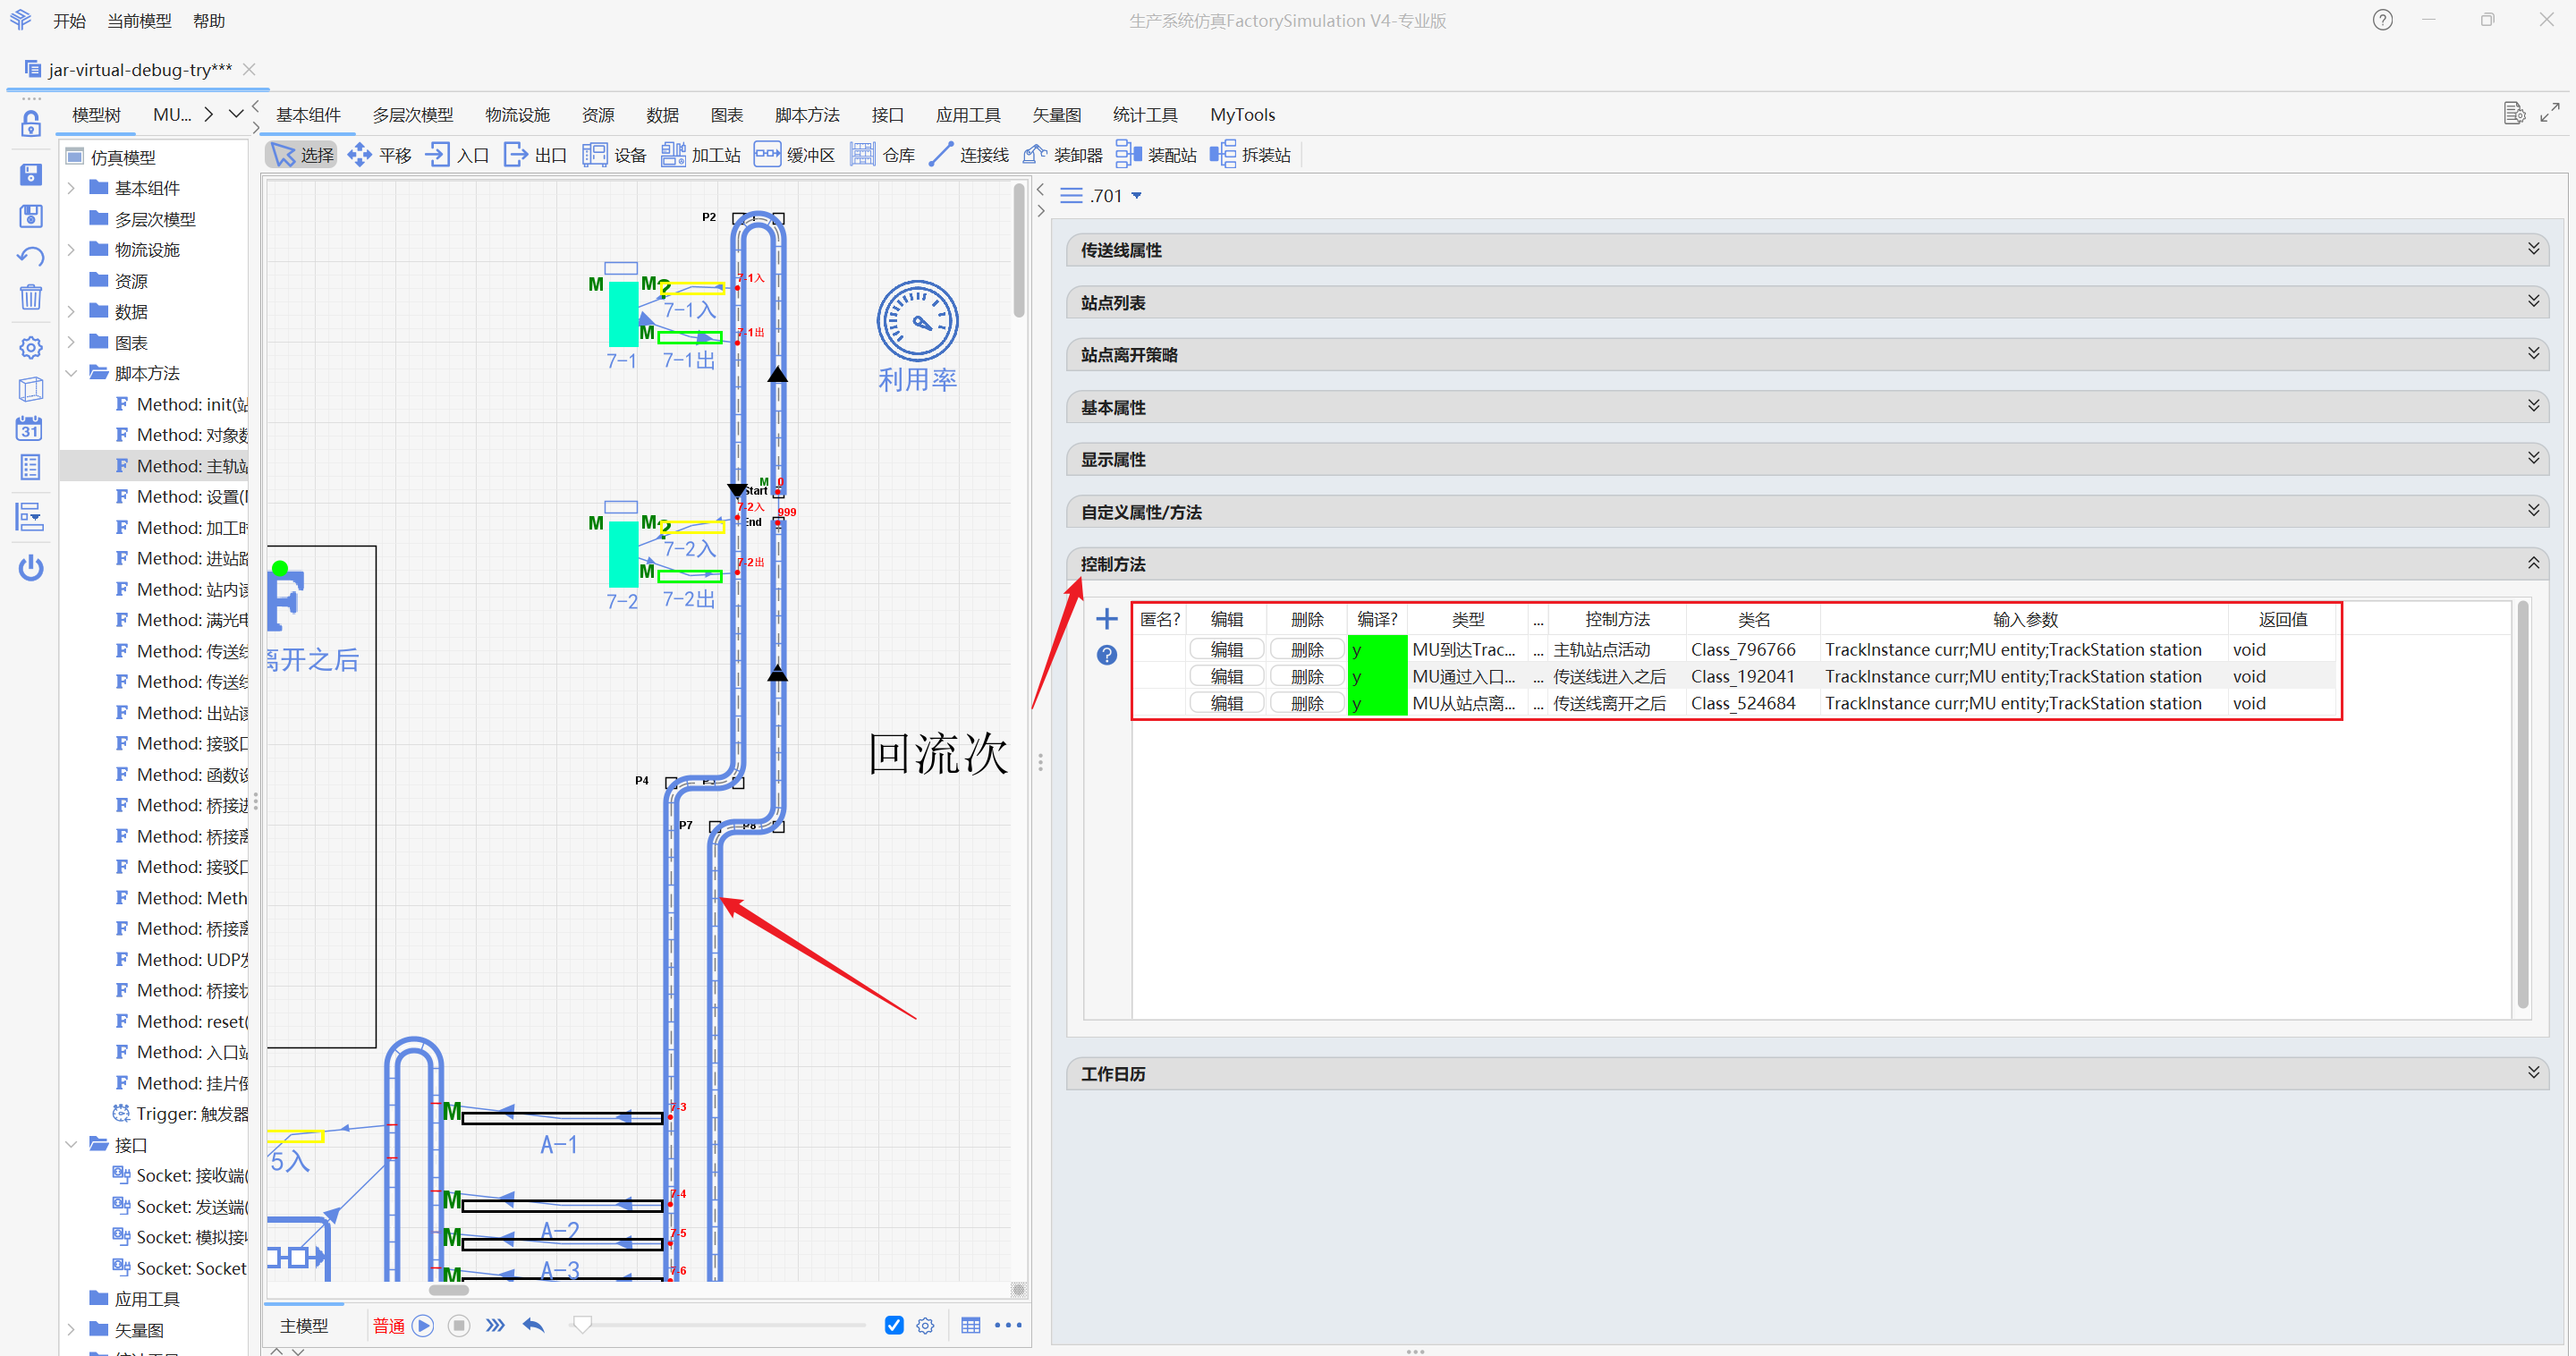
\includegraphics[width=1.0\textwidth]{pics/jack/track_method.png}
	\caption{主轨使用到的控制方法}\label{fig:track_method}
\end{figure}
\begin{enumerate}
	\item \bf{主轨站点活动}：\it{MU到达Track站点之后}调用\par 
	当前站点不是0或999，调用“进站路过事件”向控制测试桩发送进站路过消息。MU的自定义属性“nextStation”由UDP数据设置，此处取出该属性值，并用它设置MU的离开站点。然后判断该Track站点是否有离开对象（出口连接线相连），没有则设置从线尾离开（本例的线尾回绕回到线头），有则判断是否设置了满光电，满了则设置从线尾离开。
	\begin{lstlisting}
public final class Class_326161 extends MethodClass {
    public Class_326161(SimulationModel model, SimulationInstance instance, ControlMethod method) {super(model, instance, method);}
    public void 主轨站点活动(TrackInstance curr, MU entity, TrackStation station) throws Exception {
        //判断衣架是否有属性flag，没有则说明衣架第一次入轨，此时衣架需要出轨
        if(!station.getNo().equals("0") && !station.getNo().equals("999")){
           // exec("进站路过事件", curr.getSimpleNo(),station.getNo(),entity.getSimpleNo(),entity.getSimpleNo(),"0");
        }
        entity.setExitStationNo(entity.getAttribute("nextStation"));
        if(station.getNo().equals(entity.getAttribute("nextStation"))){
            if(station.getExitObjectList().size() == 0){
                // 该Track站点没有离开对象（Track站点有旁路连接线）
                entity.setExitStationNo("999");
            }else{
                MaterialFlowObjectInstance mfi = instance.findChildByID(station.getExitObjectList().get(0).getId());
                //println(mfi);
                if (mfi.hasAttribute("光电")) {
                    int flag = mfi.getAttribute("光电");
                    // 表明 容量满了！
                    if(flag == 1){
                       entity.setExitStationNo("999");
                    }
                }
            }
        }
    }
}
	\end{lstlisting}\vspace{-30pt}
	\item \bf{传送线进入之后}：\it{MU通过入口站点进入Track之后}调用\par
	此处处理MU从Track站点0进入主轨、或者从其它任何Track站点入轨（例如桥接进入主轨、存储杆出库进入主轨、工站出站进入主轨）均会触发该事件，本例中没有具体应用。以后可以根据需要添加处理。
	\item \bf{传送线离开之后}：\it{MU从站点离开Track之后}调用\par
	此处处理MU从Track站点离开主轨，离开主轨会进入工站、存储杆、桥接等。本例在此事件中发送“进站事件”消息，通知控制测试桩MU进入工站（或存储杆、桥接）。
	\begin{lstlisting}
public final class Class_802859 extends MethodClass {
    public Class_802859(SimulationModel model, SimulationInstance instance, ControlMethod method) {super(model, instance, method);}
    public void 传送线离开之后(TrackInstance curr, MU entity, TrackStation station) throws Exception {
     
            if(!station.getNo().equals("0") && !station.getNo().equals("999")){
                exec("进站路过事件", curr.getSimpleNo(),station.getNo(),entity.getSimpleNo(),entity.getSimpleNo(),"1");
                print("进站事件(传送线离开之后)："+ curr.getSimpleNo() +", "+ station.getNo() +", " + entity.getSimpleNo() +", " + entity.getSimpleNo());
            } 
    }
}
	\end{lstlisting}\vspace{-30pt}
\end{enumerate}

\subsubsection{挂片站控制方法}
\begin{enumerate}
	\item \bf{挂片倒计数}：\it{MU离开之后}\par
	功能是将当前工序任务剩余数量（processQty\footnote{\bf{processQty}：该属性为自定义属性，用于控制挂片站是否继续从螺旋弯取空衣架。}）减1。\par
	\tips{只在挂片站使用}
	\begin{figure}[H]%[htbp!]
		\centering
		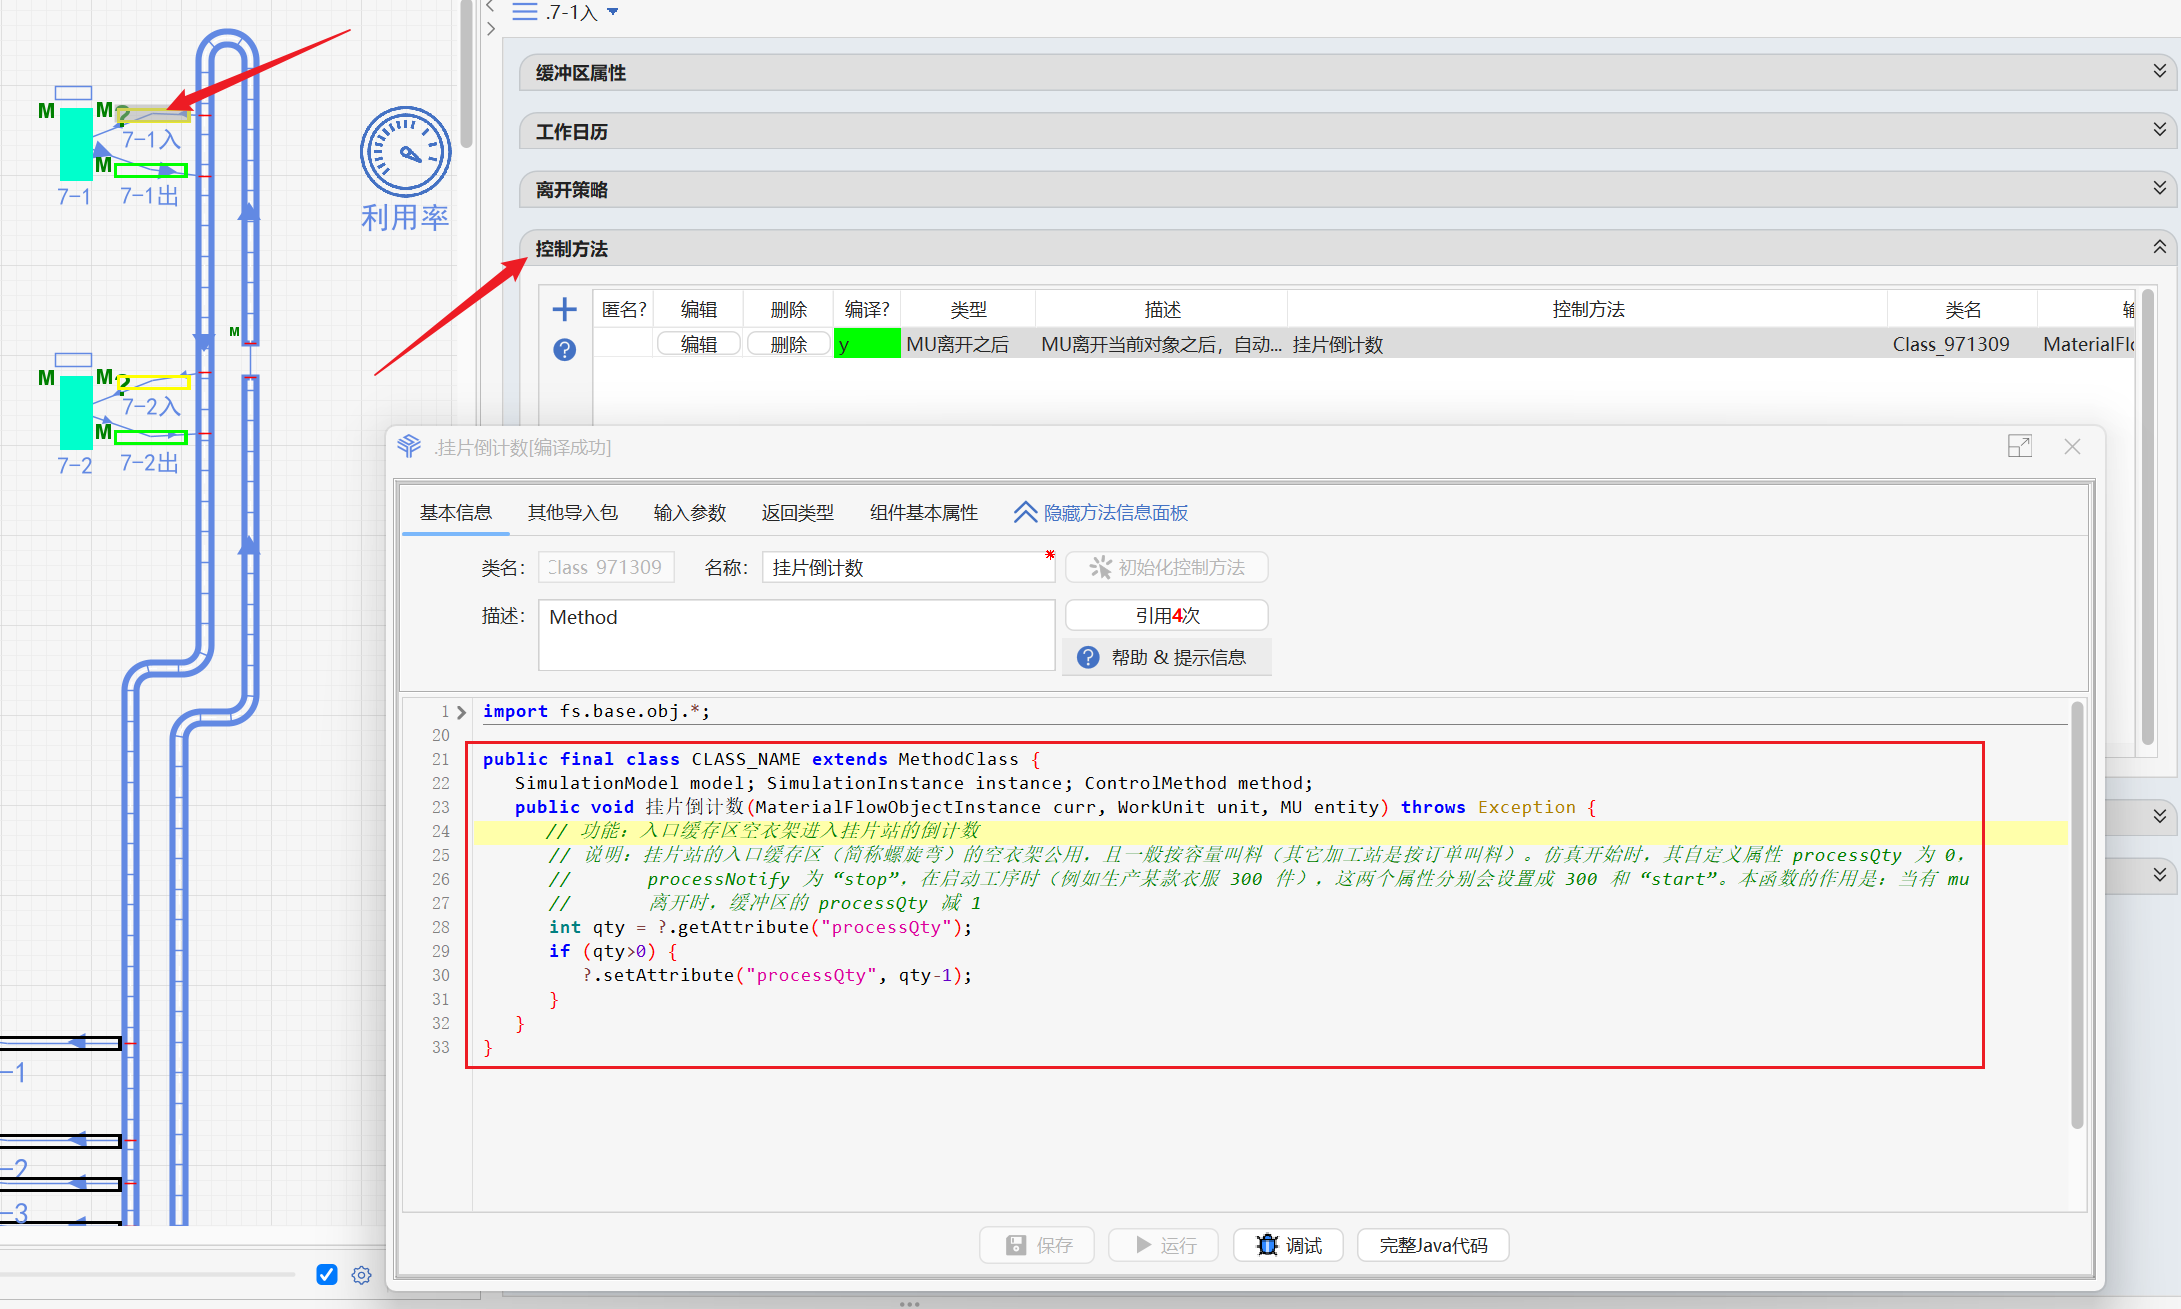
\includegraphics[width=0.8\textwidth]{pics/jack/hangering_station_buffer_method.png}
		\caption{挂片站入站缓存区MU离开之后调用\it{挂片倒计数}}\label{fig:hangering_station_buffer_method}
	\end{figure}
	\item 工站入库缓存$rightarrow$工站（\it{连接线}）\bf{通行控制}：
	\begin{figure}[H]%[htbp!]
		\centering
		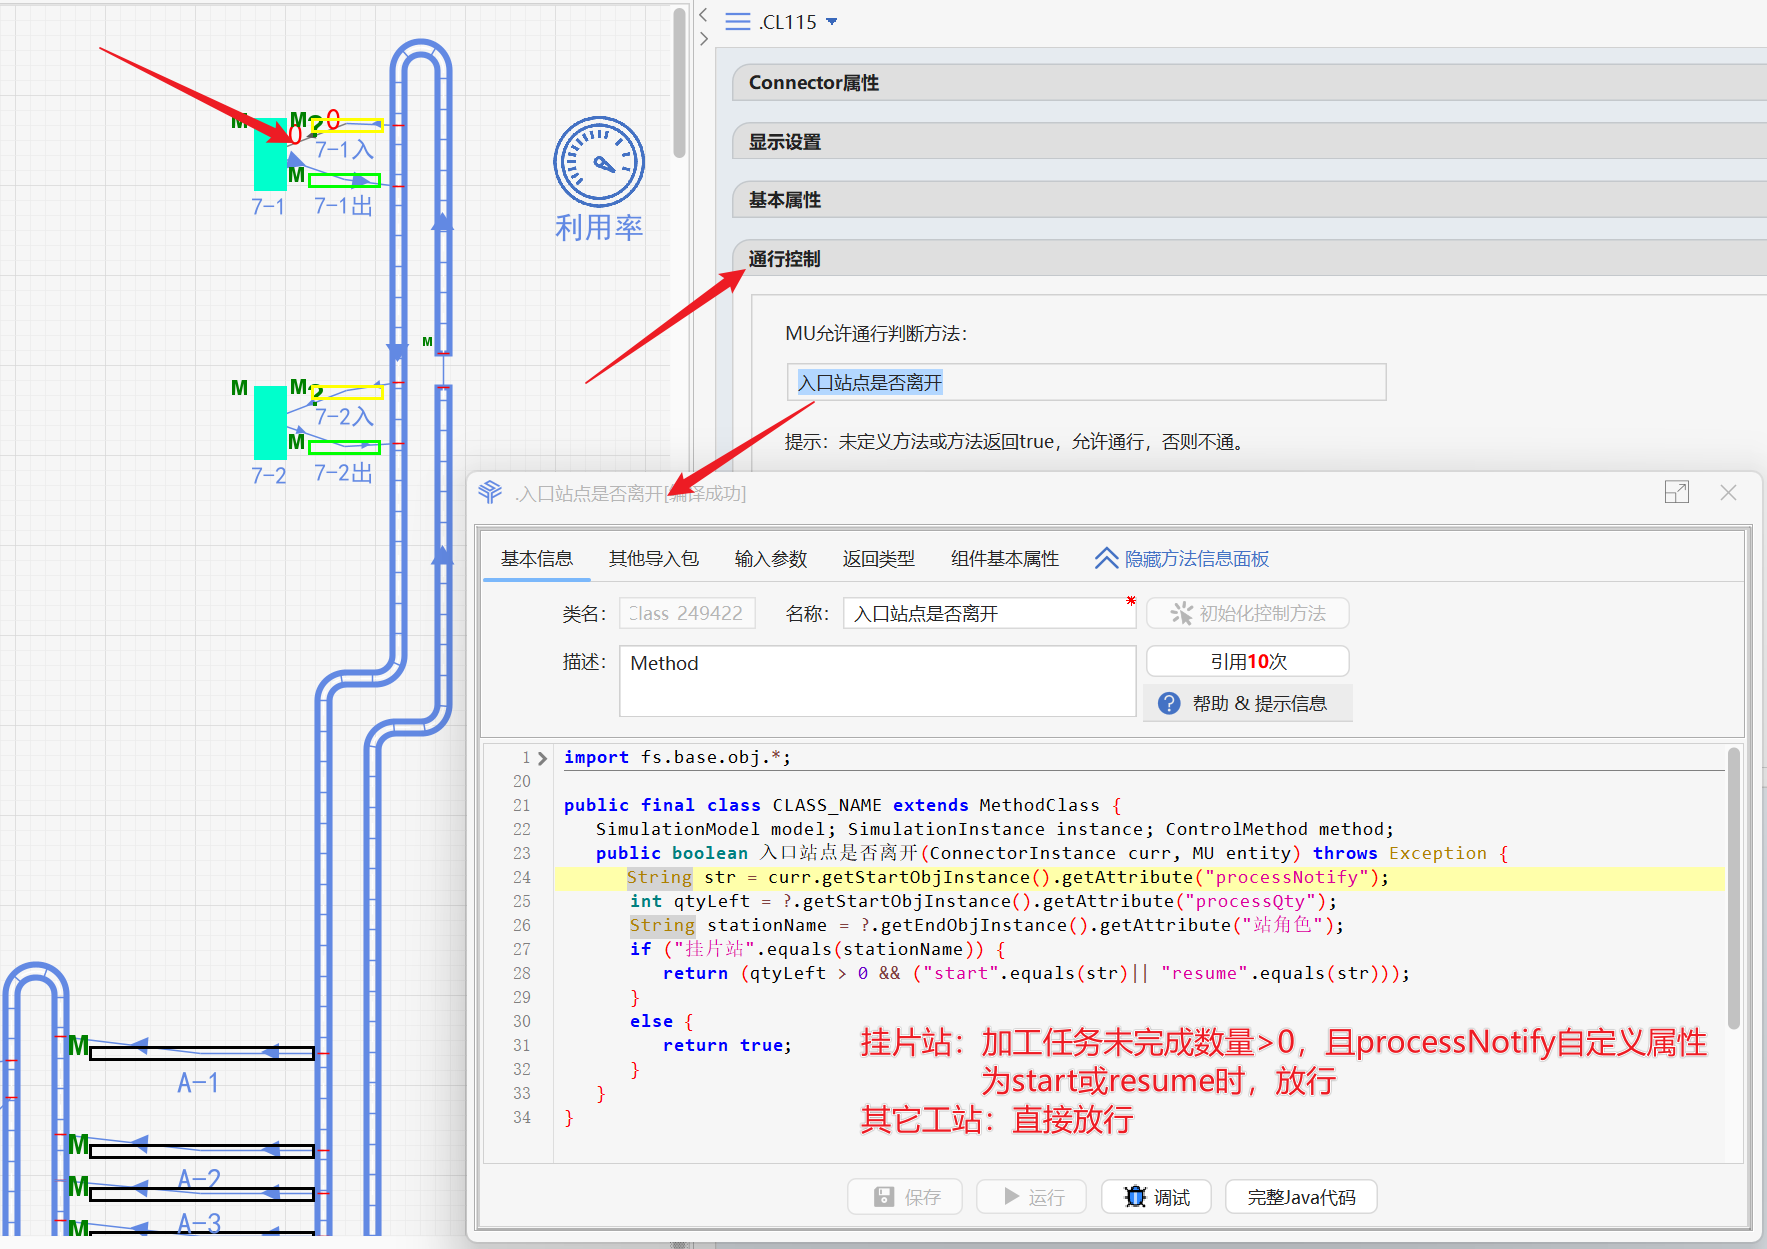
\includegraphics[width=0.8\textwidth]{pics/jack/hangering_station_buffer_passthrough.png}
		\caption{“站缓存$\rightarrow$工站”通行控制}\label{fig:hangering_station_buffer_passthrough}
	\end{figure}
	\item \bf{MU离开之后}: \it{挂片站$\rightarrow$出站缓冲区}
	\begin{figure}[H]%[htbp!]
		\centering
		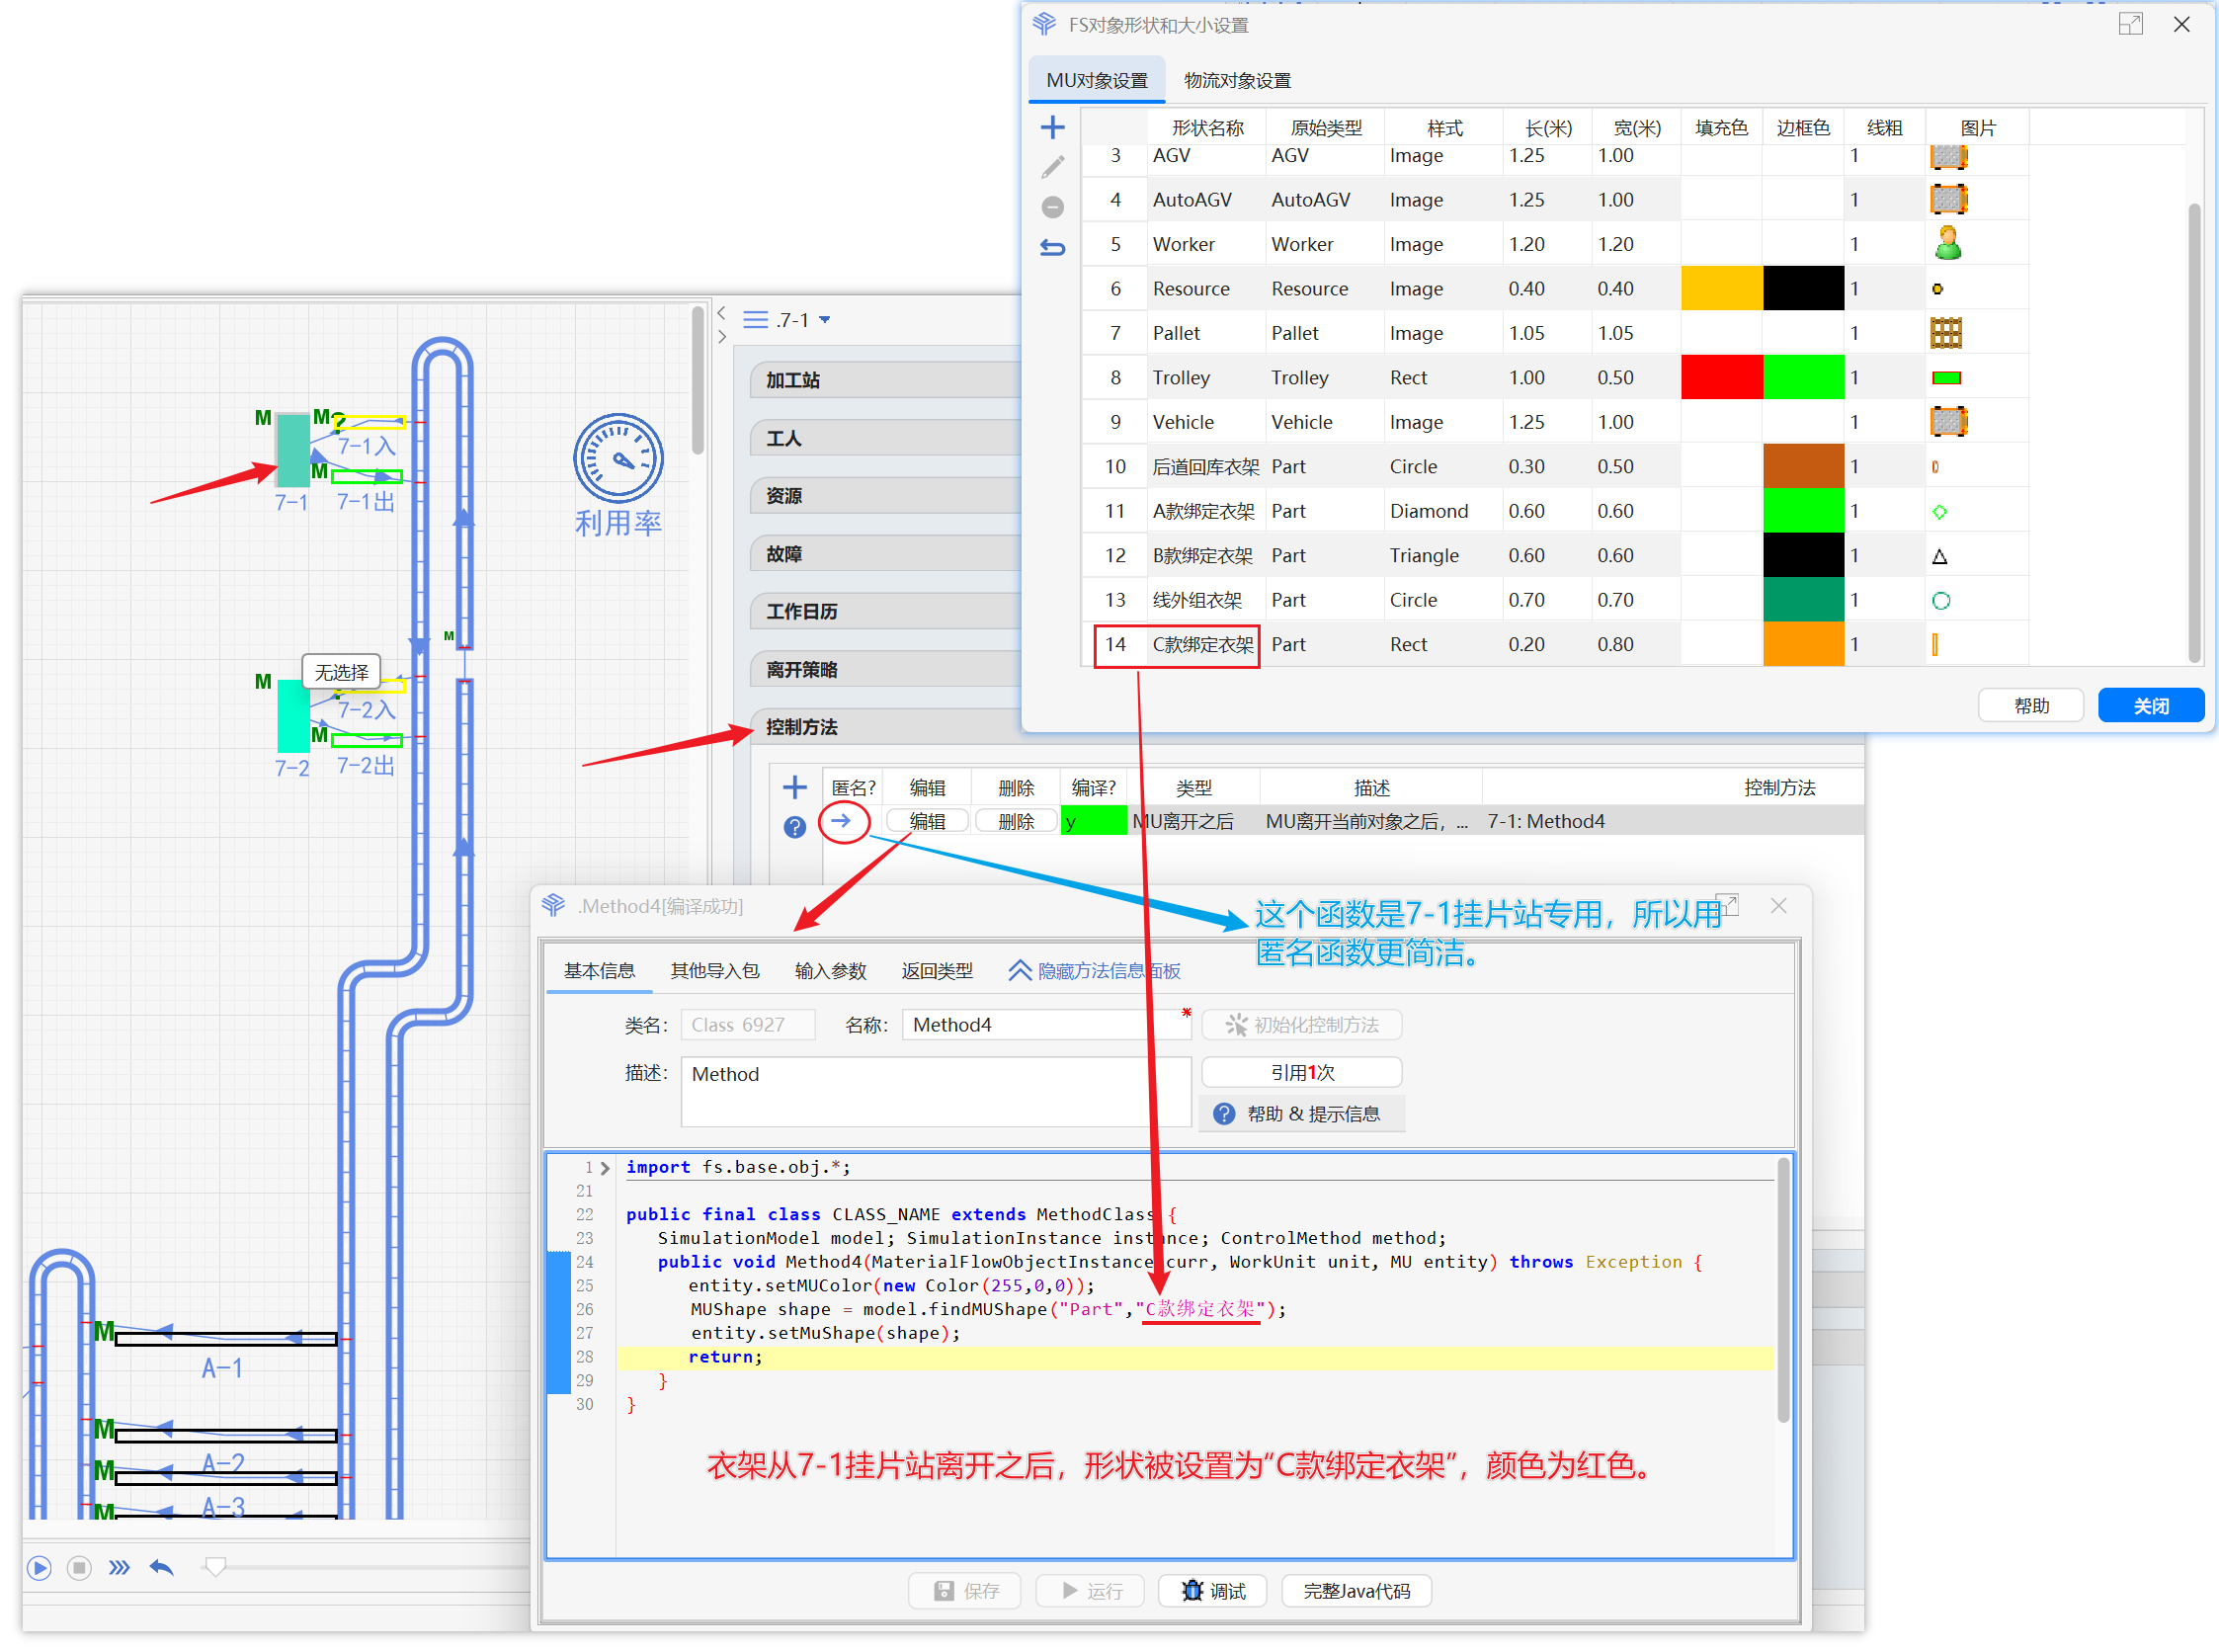
\includegraphics[width=0.8\textwidth]{pics/jack/MU_leave_7_1.png}
		\caption{MU离开挂片站}\label{fig:mu_leave_7_1}
	\end{figure}
	\item \bf{出站缓冲区控制方法}
	\begin{figure}[H]%[htbp!]
		\centering
		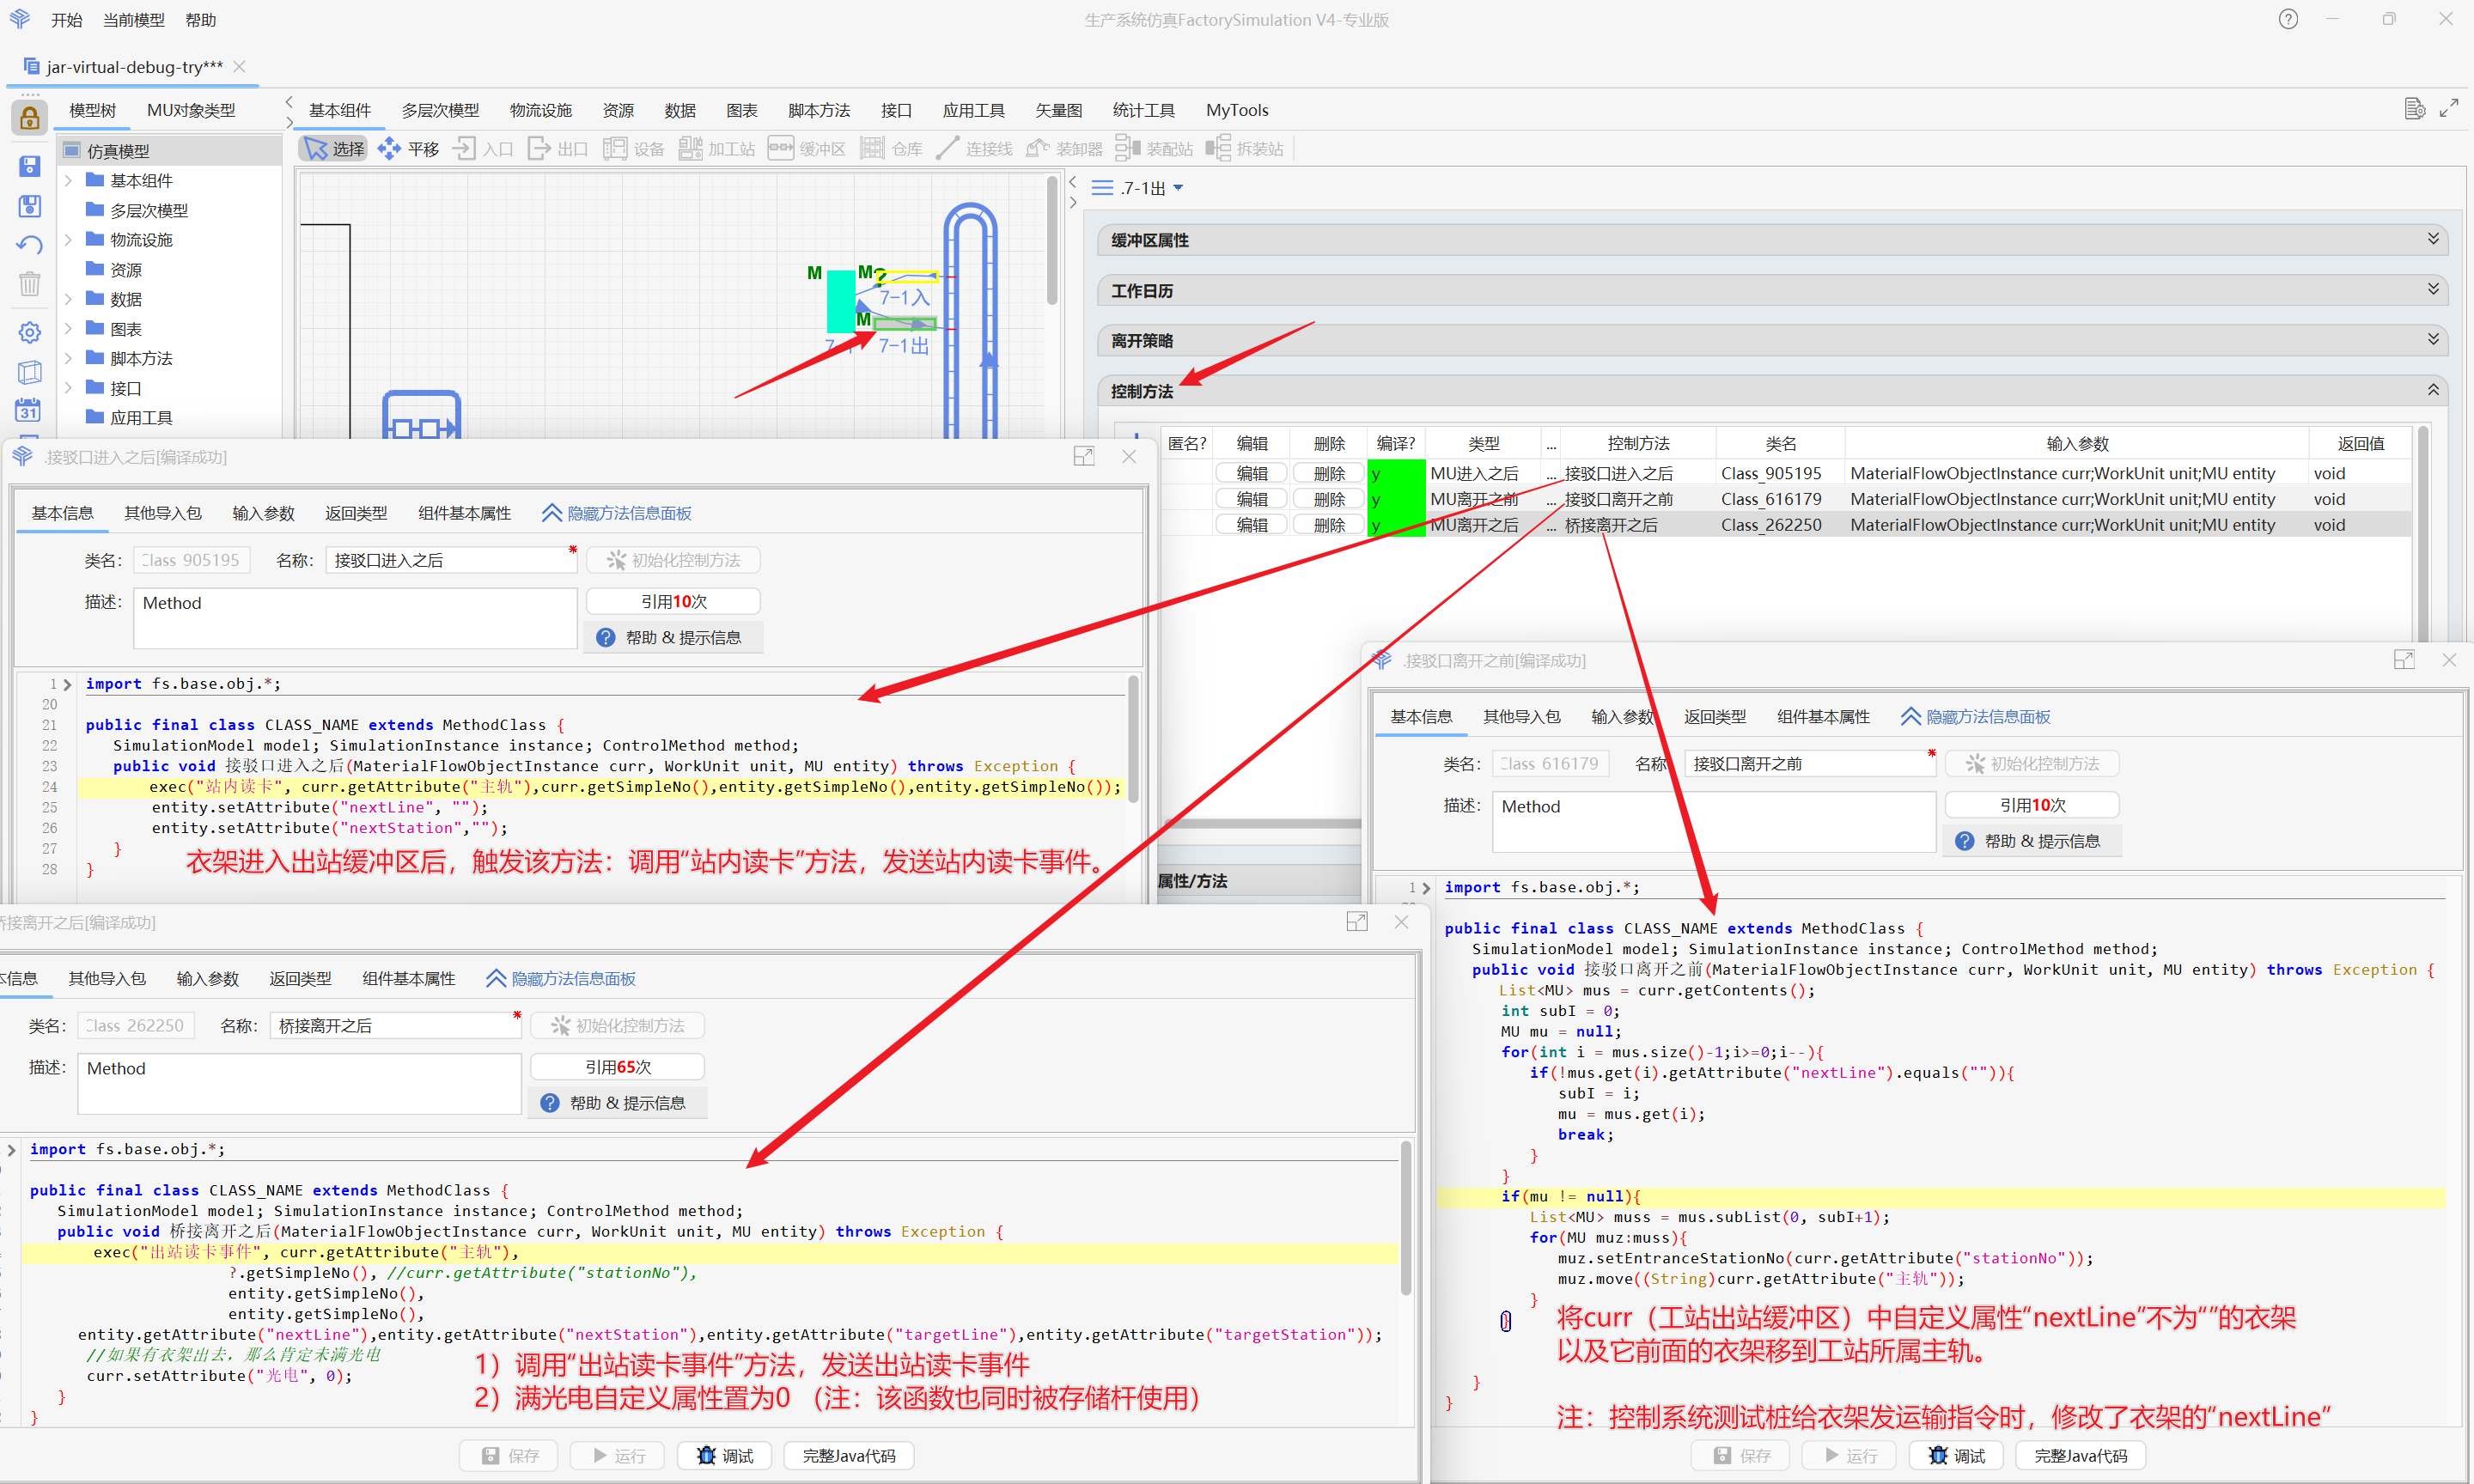
\includegraphics[width=0.8\textwidth]{pics/jack/station_exit_buffer.png}
		\caption{工站出站缓冲区的控制方法}\label{fig:station_exit_buffer}
	\end{figure}

\end{enumerate}

\subsubsection{车缝站控制方法}
\begin{enumerate}
	\item 工站入库缓存$\rightarrow$工站（\it{连接线}）\bf{通行控制}：此处的通行控制与挂片站相同，但目前的逻辑对应车缝站总是放行的（return true），可以删除。
	\item \bf{MU离开之后}: \it{车缝站$\rightarrow$出站缓冲区}：使用匿名函数，设置衣架颜色。
	\begin{lstlisting}
		...
        entity.setMUColor(new Color(255,165,0));
		...
	\end{lstlisting}\vspace{-30pt}
	\item \bf{出站缓冲区控制方法}：与挂片站引用的函数相同（见\secref{fig:station_exit_buffer}）

\end{enumerate}

\subsubsection{存储杆、桥接控制方法}
\begin{figure}[H]%[htbp!]
	\centering
	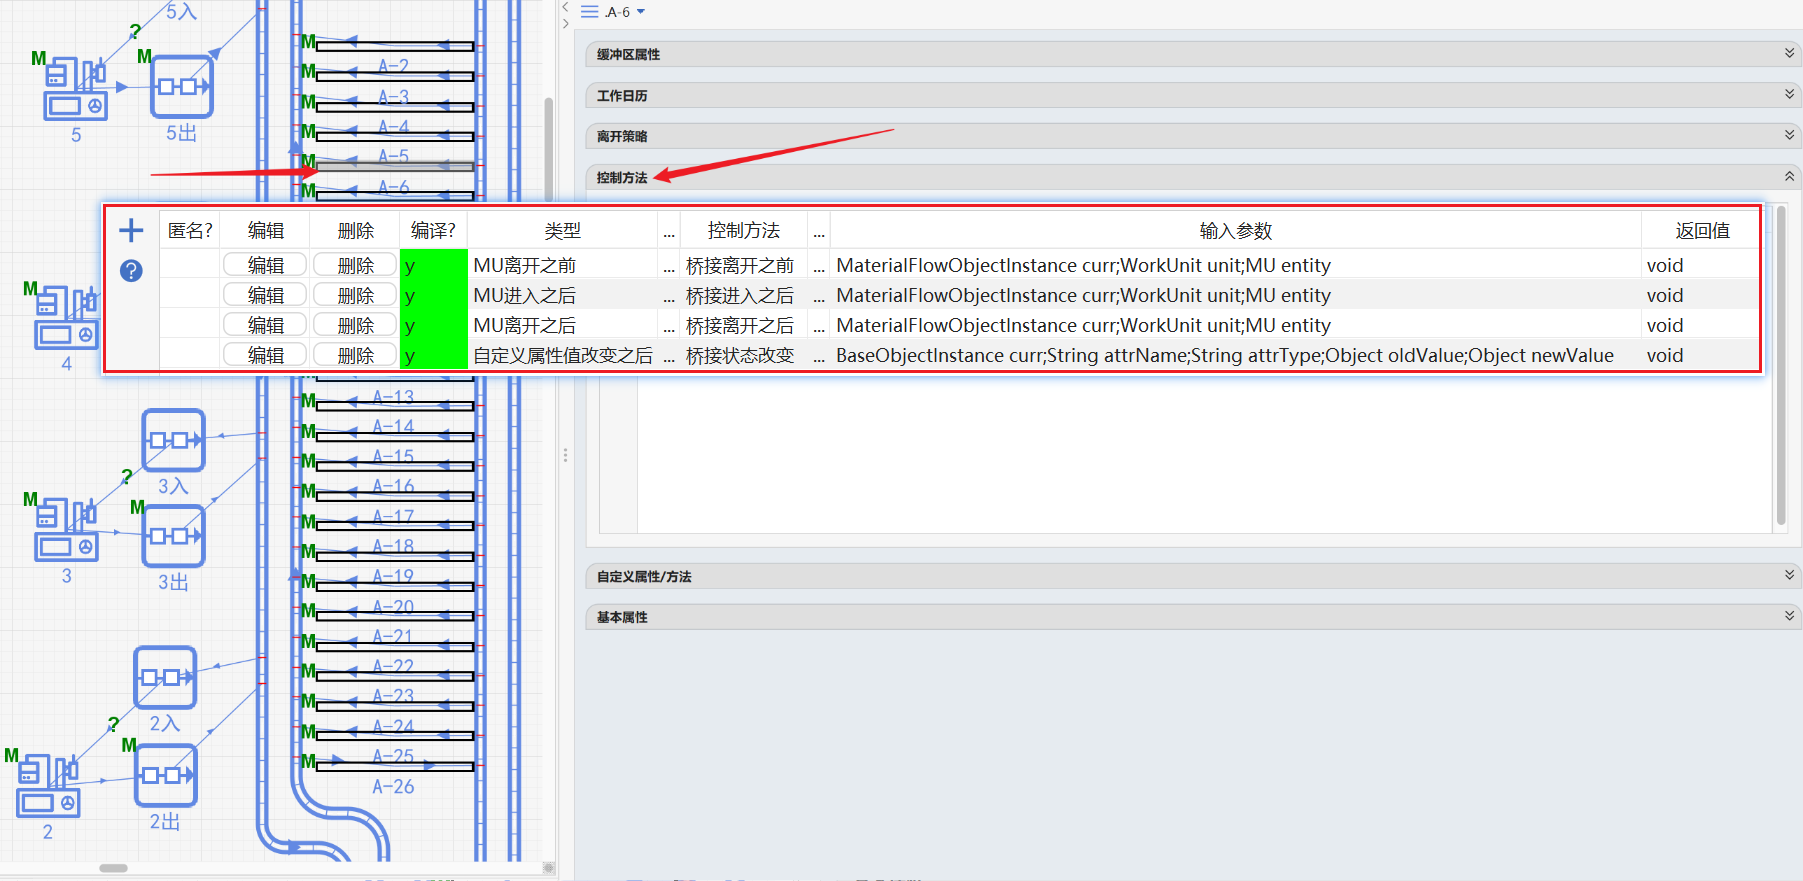
\includegraphics[width=0.6\textwidth]{pics/jack/rod_method.png}
	\caption{存储杆、回流杆和快速通道控制方法}\label{fig:rod_method}
\end{figure}
\begin{enumerate}
	\item \it{MU离开之前}：\bf{桥接离开之前}
	\begin{lstlisting}
public final class Class_448802 extends MethodClass {
    public Class_448802(SimulationModel model, SimulationInstance instance, ControlMethod method) {super(model, instance, method);}
    public void 桥接离开之前(MaterialFlowObjectInstance curr, WorkUnit unit, MU entity) throws Exception {
        List<MU> mus = curr.getContents();
        int subI = 0;
        MU mu = null;
        for(int i = mus.size()-1;i>=0;i--){
            if(!mus.get(i).getAttribute("nextLine").equals("")){
                subI = i;
                mu = mus.get(i);
                break;
            }
        }
        if(mu != null){
            List<MU> muss = mus.subList(0, subI+1);
            for(MU muz:muss){
                muz.setEntranceStationNo(curr.getAttribute("stationNo"));
                muz.move((String)curr.getAttribute("主轨"));
            }
        }
    }
}		
	\end{lstlisting}\vspace{-30pt}

	\item \it{MU进入之后}：\bf{桥接进入之后}
	\begin{lstlisting}
public final class Class_785444 extends MethodClass {
    public Class_785444(SimulationModel model, SimulationInstance instance, ControlMethod method) {super(model, instance, method);}
    public void 桥接进入之后(MaterialFlowObjectInstance curr, WorkUnit unit, MU entity) throws Exception {
        entity.setAttribute("nextLine", "");
        entity.setAttribute("nextStation","");
        // 当前mu的容量
        int size =  curr.getCapacity();
        // 容量小于等于2
        if(size - curr.size() <= 2){
            // 如果和容量相等 表明光电是1
            if(size ==  curr.size()){
                curr.setAttribute("光电", 1);
            }else{
                // 0.05 光电是1
                if( Math.random()<0.5){
                  curr.setAttribute("光电", 1);
                }
            }
        }
    }
}		
	\end{lstlisting}\vspace{-30pt}

	\item \it{MU离开之后}：\bf{桥接离开之后}
	\begin{lstlisting}
public final class Class_262250 extends MethodClass {
    public Class_262250(SimulationModel model, SimulationInstance instance, ControlMethod method) {super(model, instance, method);}
    public void 桥接离开之后(MaterialFlowObjectInstance curr, WorkUnit unit, MU entity) throws Exception {
      exec("出站读卡事件", curr.getAttribute("主轨"),
                        curr.getSimpleNo(), //curr.getAttribute("stationNo"),
                        entity.getSimpleNo(),
                        entity.getSimpleNo(),
        entity.getAttribute("nextLine"),entity.getAttribute("nextStation"),entity.getAttribute("targetLine"),entity.getAttribute("targetStation"));
         //如果有衣架出去，那么肯定未满光电
         curr.setAttribute("光电", 0);
    }
}	
	\end{lstlisting}\vspace{-30pt}

	\item \it{自定义属性值改变之后}：\bf{桥接状态改变}
	\begin{lstlisting}
public final class Class_486757 extends MethodClass {
    public Class_486757(SimulationModel model, SimulationInstance instance, ControlMethod method) {super(model, instance, method);}
    public void 桥接状态改变(BaseObjectInstance curr, String attrName, String attrType, Object oldValue, Object newValue) throws Exception {
     if(attrName.equals("光电")){
            if(oldValue != newValue){
               
               ConnectorInstance ci = ((MaterialFlowObjectInstance)curr).getPredConnectorList().get(0);
            
               Connector c = ci.getObject();
               TrackStation ts = c.getStartTrackStation();
               //exec(".满光电事件", ts.getTrack().getSimpleNo(),ts.getNo(),newValue+"");
               exec(".满光电事件", ts.getTrack().getSimpleNo(),curr.getSimpleNo(),newValue+"");
            }
         }
    }
}
	\end{lstlisting}\vspace{-30pt}
\end{enumerate}

\subsection{虚拟调试步骤}
\begin{enumerate}[label=\arabic*)]
	\item \bf{运行fs}，打开对应模型（例如“jar-virtual-debut.fs”），如之前已运行过，则重置。
	\item \bf{运行吊挂测试桩}
	\item \bf{运行控制测试桩}
	\item \bf{运行前端（吊挂测试桩前端）}
	\item \bf{打开浏览器}
	\item \bf{浏览器：初始化基础数据}：\it{节点表}、\it{桥接表}、\it{库区表}、\it{库存（工站/存储杆）}
	\item \bf{fs: 启动仿真}
	\item \bf{浏览器：排产}
\end{enumerate}
\subsection{注意事项}
\begin{enumerate}
	\item \bf{加速因子}：默认50，本例的虚拟调试建议调到300，太快了UDP可能丢包，太慢影响软件调试效率。
	\item \bf{打印日志过滤}：事件高速并发，调试程序是的日志打印太频繁，可使用LogIf类的静态方法canLog()过滤日志。
\end{enumerate}
